% Options for packages loaded elsewhere
% Options for packages loaded elsewhere
\PassOptionsToPackage{unicode}{hyperref}
\PassOptionsToPackage{hyphens}{url}
\PassOptionsToPackage{dvipsnames,svgnames,x11names}{xcolor}
%
\documentclass[
  12pt,
  letterpaper,
]{article}
\usepackage{xcolor}
\usepackage[margin=1in]{geometry}
\usepackage{amsmath,amssymb}
\setcounter{secnumdepth}{-\maxdimen} % remove section numbering
\usepackage{iftex}
\ifPDFTeX
  \usepackage[T1]{fontenc}
  \usepackage[utf8]{inputenc}
  \usepackage{textcomp} % provide euro and other symbols
\else % if luatex or xetex
  \usepackage{unicode-math} % this also loads fontspec
  \defaultfontfeatures{Scale=MatchLowercase}
  \defaultfontfeatures[\rmfamily]{Ligatures=TeX,Scale=1}
\fi
\usepackage{lmodern}
\ifPDFTeX\else
  % xetex/luatex font selection
  \setmainfont[]{Times New Roman}
\fi
% Use upquote if available, for straight quotes in verbatim environments
\IfFileExists{upquote.sty}{\usepackage{upquote}}{}
\IfFileExists{microtype.sty}{% use microtype if available
  \usepackage[]{microtype}
  \UseMicrotypeSet[protrusion]{basicmath} % disable protrusion for tt fonts
}{}
\usepackage{setspace}
\makeatletter
\@ifundefined{KOMAClassName}{% if non-KOMA class
  \IfFileExists{parskip.sty}{%
    \usepackage{parskip}
  }{% else
    \setlength{\parindent}{0pt}
    \setlength{\parskip}{6pt plus 2pt minus 1pt}}
}{% if KOMA class
  \KOMAoptions{parskip=half}}
\makeatother
% Make \paragraph and \subparagraph free-standing
\makeatletter
\ifx\paragraph\undefined\else
  \let\oldparagraph\paragraph
  \renewcommand{\paragraph}{
    \@ifstar
      \xxxParagraphStar
      \xxxParagraphNoStar
  }
  \newcommand{\xxxParagraphStar}[1]{\oldparagraph*{#1}\mbox{}}
  \newcommand{\xxxParagraphNoStar}[1]{\oldparagraph{#1}\mbox{}}
\fi
\ifx\subparagraph\undefined\else
  \let\oldsubparagraph\subparagraph
  \renewcommand{\subparagraph}{
    \@ifstar
      \xxxSubParagraphStar
      \xxxSubParagraphNoStar
  }
  \newcommand{\xxxSubParagraphStar}[1]{\oldsubparagraph*{#1}\mbox{}}
  \newcommand{\xxxSubParagraphNoStar}[1]{\oldsubparagraph{#1}\mbox{}}
\fi
\makeatother


\usepackage{longtable,booktabs,array}
\usepackage{calc} % for calculating minipage widths
% Correct order of tables after \paragraph or \subparagraph
\usepackage{etoolbox}
\makeatletter
\patchcmd\longtable{\par}{\if@noskipsec\mbox{}\fi\par}{}{}
\makeatother
% Allow footnotes in longtable head/foot
\IfFileExists{footnotehyper.sty}{\usepackage{footnotehyper}}{\usepackage{footnote}}
\makesavenoteenv{longtable}
\usepackage{graphicx}
\makeatletter
\newsavebox\pandoc@box
\newcommand*\pandocbounded[1]{% scales image to fit in text height/width
  \sbox\pandoc@box{#1}%
  \Gscale@div\@tempa{\textheight}{\dimexpr\ht\pandoc@box+\dp\pandoc@box\relax}%
  \Gscale@div\@tempb{\linewidth}{\wd\pandoc@box}%
  \ifdim\@tempb\p@<\@tempa\p@\let\@tempa\@tempb\fi% select the smaller of both
  \ifdim\@tempa\p@<\p@\scalebox{\@tempa}{\usebox\pandoc@box}%
  \else\usebox{\pandoc@box}%
  \fi%
}
% Set default figure placement to htbp
\def\fps@figure{htbp}
\makeatother


% definitions for citeproc citations
\NewDocumentCommand\citeproctext{}{}
\NewDocumentCommand\citeproc{mm}{%
  \begingroup\def\citeproctext{#2}\cite{#1}\endgroup}
\makeatletter
 % allow citations to break across lines
 \let\@cite@ofmt\@firstofone
 % avoid brackets around text for \cite:
 \def\@biblabel#1{}
 \def\@cite#1#2{{#1\if@tempswa , #2\fi}}
\makeatother
\newlength{\cslhangindent}
\setlength{\cslhangindent}{1.5em}
\newlength{\csllabelwidth}
\setlength{\csllabelwidth}{3em}
\newenvironment{CSLReferences}[2] % #1 hanging-indent, #2 entry-spacing
 {\begin{list}{}{%
  \setlength{\itemindent}{0pt}
  \setlength{\leftmargin}{0pt}
  \setlength{\parsep}{0pt}
  % turn on hanging indent if param 1 is 1
  \ifodd #1
   \setlength{\leftmargin}{\cslhangindent}
   \setlength{\itemindent}{-1\cslhangindent}
  \fi
  % set entry spacing
  \setlength{\itemsep}{#2\baselineskip}}}
 {\end{list}}
\usepackage{calc}
\newcommand{\CSLBlock}[1]{\hfill\break\parbox[t]{\linewidth}{\strut\ignorespaces#1\strut}}
\newcommand{\CSLLeftMargin}[1]{\parbox[t]{\csllabelwidth}{\strut#1\strut}}
\newcommand{\CSLRightInline}[1]{\parbox[t]{\linewidth - \csllabelwidth}{\strut#1\strut}}
\newcommand{\CSLIndent}[1]{\hspace{\cslhangindent}#1}



\setlength{\emergencystretch}{3em} % prevent overfull lines

\providecommand{\tightlist}{%
  \setlength{\itemsep}{0pt}\setlength{\parskip}{0pt}}



 


\usepackage{booktabs}
\usepackage{longtable}
\usepackage{float}
\usepackage{setspace}
\doublespacing
% PAR heading styles
\usepackage{titlesec}
% Principal subheads: 14pt bold
\titleformat{\section}{\normalfont\fontsize{14}{16}\bfseries}{\thesection}{1em}{}
% Secondary subheads: 12pt bold
\titleformat{\subsection}{\normalfont\fontsize{12}{14}\bfseries}{\thesubsection}{1em}{}
% Sub-subheads: 12pt bold italic, run-in
\titleformat{\subsubsection}[runin]{\normalfont\fontsize{12}{14}\bfseries\itshape}{\thesubsubsection}{1em}{}[.]
% Abstract formatting
\renewenvironment{abstract}{\par\bigskip\noindent\textbf{Abstract}\par\smallskip\noindent}{\par\bigskip}
% Remove section numbers
\setcounter{secnumdepth}{0}
\makeatletter
\@ifpackageloaded{caption}{}{\usepackage{caption}}
\AtBeginDocument{%
\ifdefined\contentsname
  \renewcommand*\contentsname{Table of contents}
\else
  \newcommand\contentsname{Table of contents}
\fi
\ifdefined\listfigurename
  \renewcommand*\listfigurename{List of Figures}
\else
  \newcommand\listfigurename{List of Figures}
\fi
\ifdefined\listtablename
  \renewcommand*\listtablename{List of Tables}
\else
  \newcommand\listtablename{List of Tables}
\fi
\ifdefined\figurename
  \renewcommand*\figurename{Figure}
\else
  \newcommand\figurename{Figure}
\fi
\ifdefined\tablename
  \renewcommand*\tablename{Table}
\else
  \newcommand\tablename{Table}
\fi
}
\@ifpackageloaded{float}{}{\usepackage{float}}
\floatstyle{ruled}
\@ifundefined{c@chapter}{\newfloat{codelisting}{h}{lop}}{\newfloat{codelisting}{h}{lop}[chapter]}
\floatname{codelisting}{Listing}
\newcommand*\listoflistings{\listof{codelisting}{List of Listings}}
\makeatother
\makeatletter
\makeatother
\makeatletter
\@ifpackageloaded{caption}{}{\usepackage{caption}}
\@ifpackageloaded{subcaption}{}{\usepackage{subcaption}}
\makeatother
\usepackage{bookmark}
\IfFileExists{xurl.sty}{\usepackage{xurl}}{} % add URL line breaks if available
\urlstyle{same}
\hypersetup{
  pdftitle={When Velocity Matters: A Contingent Capacity Framework for Disaster Recovery Administration},
  colorlinks=true,
  linkcolor={blue},
  filecolor={Maroon},
  citecolor={Blue},
  urlcolor={Blue},
  pdfcreator={LaTeX via pandoc}}


\title{When Velocity Matters: A Contingent Capacity Framework for
Disaster Recovery Administration}
\author{}
\date{}
\begin{document}
\maketitle


\setstretch{2}
\subsection*{Abstract}\label{abstract}
\addcontentsline{toc}{subsection}{Abstract}

Administrative capacity effects on program outcomes are typically
assumed to be universal. Analysis of 152 CDBG-DR grantee-disaster pairs
reveals that spending velocity---the quarterly rate of fund
expenditure---predicts recovery completion in highly context-dependent
ways. Meta-analysis of 16 velocity effect estimates shows a median
hazard ratio of 4.60, but effects range from null (housing programs,
HR=0.82) to extreme (wildfire disasters, HR=51.09). Velocity effects
concentrate in contexts where time constraints bind and capacity
substitutes are absent: wildfire disasters requiring completion before
next fire season (HR=51.09), administration programs lacking fixed
construction timelines (HR=30.74), late program phases facing closeout
deadlines (HR=5.00), and novice grantees without institutional
alternatives (HR=4.61). These findings support a contingent capacity
framework: administrative capacity is not universally beneficial but
depends on disaster urgency, program type, lifecycle phase, and
organizational experience. Policy implications favor targeted
interventions in high-leverage contexts over universal
capacity-building.

\subsection*{Evidence for Practice}\label{evidence-for-practice}
\addcontentsline{toc}{subsection}{Evidence for Practice}

\begin{itemize}
\tightlist
\item
  \textbf{Prioritize wildfire programs}: Spending velocity has 10x
  stronger effects on wildfire recovery (HR=51.09) than hurricanes
  (HR=4.58), justifying intensive technical assistance for fire-affected
  communities
\item
  \textbf{Focus on administration programs}: Velocity most strongly
  predicts completion for planning and capacity-building activities
  (HR=30.74), not physical construction
\item
  \textbf{Invest in late-phase support}: Late-stage velocity (HR=5.00)
  matters more than early planning velocity (HR=2.04), suggesting
  closeout assistance deserves priority
\item
  \textbf{Target novice grantees}: First-time CDBG-DR recipients depend
  more on velocity (HR=4.61) than experienced grantees (HR=3.15), who
  have institutional alternatives
\item
  \textbf{Implement differentiated monitoring}: Allocate 60\% of
  technical assistance to high-leverage contexts (wildfire,
  administration, novice) rather than uniform monitoring
\end{itemize}

\section{Introduction}\label{introduction}

Federal disaster recovery programs face persistent completion
challenges. The Community Development Block Grant-Disaster Recovery
(CDBG-DR) program, which has distributed over \$90 billion since 1993,
exhibits substantial variation in completion timing, with some programs
achieving 95\% expenditure within five years while others remain
incomplete after two decades (U.S. Government Accountability Office
2019; HUD Office of Inspector General 2021). Understanding what
administrative factors accelerate recovery completion remains a central
question for disaster policy.

Administrative capacity---the ability of government organizations to
effectively implement policy---has emerged as a key explanatory factor
(Wu et al. 2015; Christensen and Liang 2017). Prior research identifies
multiple capacity dimensions including human capital, organizational
resources, and management practices (Ingraham and Donahue 2000; Painter
and Pierre 2002). In disaster contexts, financial management
capacity---particularly the ability to rapidly obligate, disburse, and
expend recovery funds---appears especially consequential (Gerber and
Robinson 2022; Smith and Martin 2021).

However, existing research typically treats capacity effects as
universal: more capacity is assumed to improve outcomes regardless of
context. This assumption may obscure important heterogeneity. If
capacity effects vary by disaster type, program characteristics, or
organizational experience, uniform capacity-building interventions may
be poorly targeted.

This analysis investigates spending velocity---the quarterly rate at
which grantees expend CDBG-DR funds---as an operational capacity
measure. Three research questions guide the investigation: (1) When
during the program lifecycle does velocity matter most? (2) Where across
disaster and program types are velocity effects strongest? (3) Why do
velocity effects vary, and what mechanisms explain observed
heterogeneity?

Findings support a contingent capacity framework. Velocity effects are
not universal but concentrate in contexts where two conditions hold:
time constraints bind (limiting the value of slow, steady progress) and
capacity substitutes are absent (preventing alternative pathways to
completion). Wildfire disasters, administration programs, late program
phases, and novice grantees exhibit the strongest velocity effects
because they combine time pressure with limited alternatives.

The theoretical contribution lies in demonstrating that administrative
capacity effects are contingent on context. Rather than assuming linear,
universal benefits, public administration research should identify
boundary conditions and moderators that determine when capacity
investments yield returns. The policy contribution is equally direct:
velocity-enhancing interventions should concentrate on high-leverage
contexts---wildfire recovery, administrative programs, closeout phases,
and first-time grantees---rather than applying uniform capacity-building
across all disaster recovery programs.

\section{Literature Review}\label{literature-review}

\subsection{Recovery as a Multi-Sector Governance
Process}\label{recovery-as-a-multi-sector-governance-process}

Disaster recovery represents a prolonged, multi-dimensional governance
process---not a discrete ``rebuilding'' phase. Foundational disaster
scholarship emphasizes that recovery includes re-establishing housing,
livelihoods, public services, and social networks while institutions are
disrupted and priorities are contested (Quarantelli 1999). Planning and
disaster research further underscores that recovery decision-making is
``time-compressed'': urgent actions (temporary shelter, debris removal,
safety repairs) occur alongside long-horizon choices about land use,
infrastructure systems, and redevelopment, often before damages and
needs are fully known (Olshansky et al. 2012; Zhang and Peacock 2019).
International policy frameworks reinforce this governance lens by
defining recovery as a moment to reduce future risk and ``build back
better,'' requiring coordination across sectors and levels of government
(United Nations Office for Disaster Risk Reduction 2015).

From a comparative standpoint, recovery governance is interdependent:
national governments, subnational authorities, private contractors,
civil society organizations, and international donors frequently control
different resources and approvals, producing long decision chains and
multiple accountability relationships. Post-disaster needs assessments
and recovery strategies are intended to create a shared evidence base,
align priorities, and coordinate financing across actors (Global
Facility for Disaster Reduction and Recovery 2013). Yet this model also
highlights a persistent tension: recovery systems must accelerate action
while maintaining fiduciary controls, transparency, and legitimacy, all
of which can slow implementation.

\subsection{Financing Long-Term
Recovery}\label{financing-long-term-recovery}

Long-term recovery is typically financed through layered streams
(insurance, loans, philanthropic funding, and public transfers) that
arrive at different speeds and operate under different rules. Where
governments rely on discretionary recovery funds---block grants, special
reconstruction funds, or donor-financed recovery packages---program
design often trades flexibility for intensified reporting, procurement,
and compliance requirements intended to safeguard public resources and
target assistance. In the U.S. context, this tradeoff is particularly
visible in the Community Development Block Grant--Disaster Recovery
(CDBG-DR) mechanism: supplemental appropriations administered through
HUD's CDBG authorities are repeatedly created to meet unmet recovery
needs, but each appropriation can arrive with distinct statutory
directions and implementing requirements, complicating program design
and startup (Jaroscak 2020).

Because CDBG-DR is structured as a flexible block grant, grantees have
broad discretion to tailor activities to local needs; at the same time,
discretion is paired with extensive planning, documentation, and
monitoring expectations. Oversight bodies consistently describe
performance challenges that follow from this design, including long
delays between allocation, program launch, and closeout---often linked
to procurement, environmental review, and the establishment of
administrative systems capable of handling eligibility determinations,
construction management, and payments (U.S. Government Accountability
Office 2019; U.S. Department of Housing and Urban Development 2020).

\subsection{Capacity and
Implementation}\label{capacity-and-implementation}

A central claim across disaster recovery and public administration
research is that capacity shapes both the speed and distribution of
recovery. Capacity is multidimensional. In public policy scholarship,
``policy capacity'' is frequently defined as a bundle of analytical,
operational, and political competences and capabilities at individual,
organizational, and system levels (Wu et al. 2015). This framework maps
well to recovery: governments must (1) produce credible needs
assessments and priorities (analytical), (2) translate plans into
contracts, reimbursements, and completed projects through procurement
and financial systems (operational), and (3) sustain legitimacy and
coalitional support under high stress and conflict over redevelopment
choices (political).

Disaster-focused research aligns with this view by showing that
institutional arrangements and administrative resources (staffing,
expertise, and organizational experience) are associated with resilience
and recovery performance (Gerber and Robinson 2022). Recovery also
depends on intergovernmental and cross-sector networks, where
coordination and information sharing can substitute for hierarchical
authority but require deliberate relationship management and
trust-building (Kapucu 2009; Jr. and Streib 2006).

Beyond disaster-specific literature, intergovernmental grants research
provides a complementary lens: administrative capacity influences not
only whether jurisdictions secure grants, but whether they can absorb
them---converting awards into implemented projects and spent funds.
Research links political and administrative capacity to federal grant
flows into local areas (Hall 2008) and shows that administrative
capacity can shape the pace of utilizing awarded funds during
time-bounded program rollouts (Shybalkina 2024). Related evidence from
high-stakes, time-sensitive federal programs indicates that
implementation timing depends on both the clarity of federal guidance
and the recipient's administrative capacity to stand up processes,
contract quickly, and manage compliance (Carley et al. 2015; Terman and
Feiock 2015).

\subsection{Contingency Theory and Context-Dependent Capacity
Effects}\label{contingency-theory-and-context-dependent-capacity-effects}

Despite extensive research linking capacity to recovery outcomes,
existing work typically treats capacity effects as universal: more
capacity is assumed to improve outcomes regardless of context. Classical
contingency theory challenges this assumption, arguing that
organizational effectiveness depends on alignment between organizational
characteristics and environmental conditions (Donaldson 2001; Burns and
Stalker 1961). Mechanistic structures suit stable environments while
organic structures suit dynamic environments (Lawrence and Lorsch 1967).
The theory implies that ``best practices'' are contextual: what works in
one environment may fail in another.

Applied to administrative capacity, contingency theory suggests that
capacity effects should vary by task characteristics. Simple, repetitive
tasks may benefit less from additional capacity than complex, uncertain
tasks (Galbraith 1973). Similarly, capacity investments may yield higher
returns when time constraints create urgency than when extended
timelines permit slower progress. This contingent perspective implies
that capacity effects should depend on: (1) task complexity and
uncertainty, (2) time constraints and urgency, (3) availability of
substitute resources, and (4) lifecycle phase and organizational
learning.

Organizational learning theory provides additional nuance. Repeated
exposure to similar tasks should improve performance (Argote and
Miron-Spektor 2011; Levitt and March 1988). Experienced grantees may
have developed institutional knowledge, established vendor
relationships, and accumulated political capital that substitute for
other capacity dimensions. Novice grantees, lacking these alternatives,
may depend more heavily on operational throughput measures like spending
velocity.

\subsection{Mechanisms That Delay or Accelerate
Recovery}\label{mechanisms-that-delay-or-accelerate-recovery}

Housing recovery programs often sit at the intersection of intense
public pressure, stringent compliance regimes, and disrupted supply
chains. Planning research identifies recurring bottlenecks: procurement
and contracting rules, permitting and environmental review requirements,
contractor scarcity, and administrative constraints embedded in program
design (Smith and Martin 2021; Zhang and Peacock 2019). These
constraints are especially salient for complex activities (multifamily
development, major rehabilitation) that require multiple rounds of
approvals, layered financing, and specialized technical capacity.

Program-level evidence also underscores how strongly startup capacity
influences downstream disbursement and completion. A large review of
CDBG-DR housing activities finds substantial delays between disasters
and the point at which housing activities begin distributing funds, with
wide variation across disasters and program types (U.S. Department of
Housing and Urban Development, Office of Policy Development and Research
2021). Oversight work similarly flags program startup as a critical
bottleneck and highlights that progress reporting can be difficult to
interpret for oversight and transparency, limiting the ability to detect
``stuck'' milestones and intervene (U.S. Government Accountability
Office 2022).

Disaster characteristics also shape recovery trajectories in systematic
ways. Hurricane recovery unfolds over years as communities rebuild
housing and infrastructure (Peacock et al. 2022). Wildfire recovery
faces different constraints: seasonal fire risk creates urgency to
complete rebuilding before the next fire season, and destroyed
structures often cannot be rebuilt in identical locations due to updated
fire codes (Mockrin et al. 2015; Kramer et al. 2019).

\subsection{Equity and the Consequences of
Delay}\label{equity-and-the-consequences-of-delay}

Recovery speed is not merely a technical performance metric; it has
distributional consequences. Delays can lengthen displacement, increase
out-of-pocket costs, and widen gaps between households with access to
insurance or credit and those reliant on public assistance. Empirical
work shows that post-disaster spending patterns can exacerbate
inequality, with disadvantaged communities often facing greater barriers
and delayed access to recovery resources (Howell and Elliott 2019).
Research on disaster housing assistance similarly finds evidence of
inequitable recovery outcomes across programs and populations, raising
concerns that administrative processes and eligibility rules can
translate into unequal benefits and uneven timelines (Peacock et al.
2022). Broader analyses of recovery funding distribution further
highlight persistent inequities relative to vulnerability, reinforcing
that administrative choices---allocation formulas, documentation
requirements, and program design---shape who benefits and how quickly
(Emrich et al. 2020).

\subsection{Measuring Recovery Pace with Duration
Models}\label{measuring-recovery-pace-with-duration-models}

Despite a large qualitative and case-based literature on recovery
governance, empirically measuring recovery ``pace'' remains difficult.
Many studies rely on audits, descriptive dashboards, or case studies
that illuminate mechanisms but limit comparative generalization (Smith
and Martin 2021; U.S. Government Accountability Office 2019).
Quantitative analyses often use cross-sectional or panel regressions to
relate recovery outcomes to capacity, hazard severity, or socioeconomic
conditions, but these approaches can implicitly exclude incomplete
programs---precisely the cases most informative about delay dynamics.

Duration models provide a strong methodological fit because they
explicitly model time to reach milestones (substantial expenditure,
project completion) and can incorporate right-censored observations
(programs not complete at the time of analysis). Event history and
survival analysis are well established in the social sciences for
studying policy adoption, implementation timing, and institutional
change (Box-Steffensmeier and Jones 2004). Applying these methods to
disaster recovery finance helps address a core inferential problem in
recovery research: many programs remain active for years, so excluding
ongoing cases can bias estimates and reduce external validity.

This methodological and conceptual landscape points to an important
empirical agenda: operationalizing capacity as implementation throughput
(spending velocity), testing whether velocity effects vary
systematically across contexts, and linking those measures to the timing
of recovery spending milestones using methods designed for time-to-event
data.

\section{Data and Methods}\label{data-and-methods}

\subsection{The CDBG-DR Program}\label{the-cdbg-dr-program}

The Community Development Block Grant-Disaster Recovery (CDBG-DR)
program represents the primary federal mechanism for long-term disaster
recovery funding in the United States. Administered by the Department of
Housing and Urban Development (HUD), CDBG-DR provides flexible block
grants to state and local governments following presidentially-declared
disasters. Unlike immediate emergency response programs such as FEMA
Public Assistance, CDBG-DR funds address unmet recovery needs that
emerge after insurance payments and other federal assistance have been
exhausted, typically focusing on housing rehabilitation, infrastructure
repair, and economic revitalization (U.S. Department of Housing and
Urban Development, Office of Policy Development and Research 2021).

The program operates through a multi-stage financial pipeline. Congress
appropriates disaster-specific funding, HUD allocates funds to eligible
grantees based on damage assessments, grantees develop action plans
detailing intended activities, HUD approves plans and obligates funds,
grantees draw down (disburse) funds as projects progress, and grantees
expend funds on eligible activities. Each stage creates potential
delays, and the pace at which funds move through this
pipeline---particularly from disbursement to final
expenditure---reflects organizational capacity to manage complex
recovery programs (Jaroscak 2020).

Grantees must submit Quarterly Performance Reports (QPRs) to HUD
documenting financial progress and activity status. These standardized
reports provide the foundation for systematic analysis of recovery
implementation timing across disasters and jurisdictions.

\subsection{Sample and Data Sources}\label{sample-and-data-sources}

Analysis draws on CDBG-DR Quarterly Performance Report data spanning
2003-2023, representing two decades of disaster recovery administration.
The dataset contains 130,605 quarterly observations across 152
grantee-disaster pairs from 78 unique jurisdictions. This sample
includes all CDBG-DR allocations with sufficient reporting history to
construct velocity measures and assess completion status.

The sample reflects the diversity of CDBG-DR administration. Government
type is roughly balanced: 37 state governments (47\%) and 40 local
governments (53\%) serve as grantees. State governments typically manage
larger allocations and coordinate recovery across multiple
jurisdictions, while local governments administer programs focused on
their own communities. Prior research suggests these administrative
contexts create different capacity dynamics (Carley et al. 2015; Terman
and Feiock 2015).

table~\ref{tbl-descriptives} presents descriptive statistics for key
sample characteristics, and figure~\ref{fig-sample-composition}
visualizes the distribution across disaster types, program types, and
government levels.

\begin{longtable}[]{@{}ll@{}}

\caption{\label{tbl-descriptives}Sample Descriptive Statistics}

\tabularnewline

\toprule\noalign{}
Characteristic & Value \\
\midrule\noalign{}
\endhead
\bottomrule\noalign{}
\endlastfoot
\textbf{Sample Size} & \\
Grantee-disaster pairs & 152 \\
Unique jurisdictions & 78 \\
Quarterly observations & 130,605 \\
\textbf{Government Type} & \\
State governments & 37 (48\%) \\
Local governments & 40 (52\%) \\
\textbf{Disaster Type} & \\
Hurricane & 77 (51\%) \\
Wildfire/Fire & 27 (18\%) \\
Other (flood, storms) & 48 (32\%) \\
\textbf{Primary Program Type} & \\
Housing & 50 (33\%) \\
Infrastructure & 56 (37\%) \\
Administration & 34 (22\%) \\
Other & 12 (8\%) \\
\textbf{Completion Status (95\%)} & \\
Complete & 41 (27.0\%) \\
Right-censored (ongoing) & 111 (73.0\%) \\
\textbf{Velocity (pp/quarter)} & \\
Mean & 1.78 \\
Median & 0.87 \\
Standard deviation & 22.6 \\

\end{longtable}

\begin{figure}

\centering{

\pandocbounded{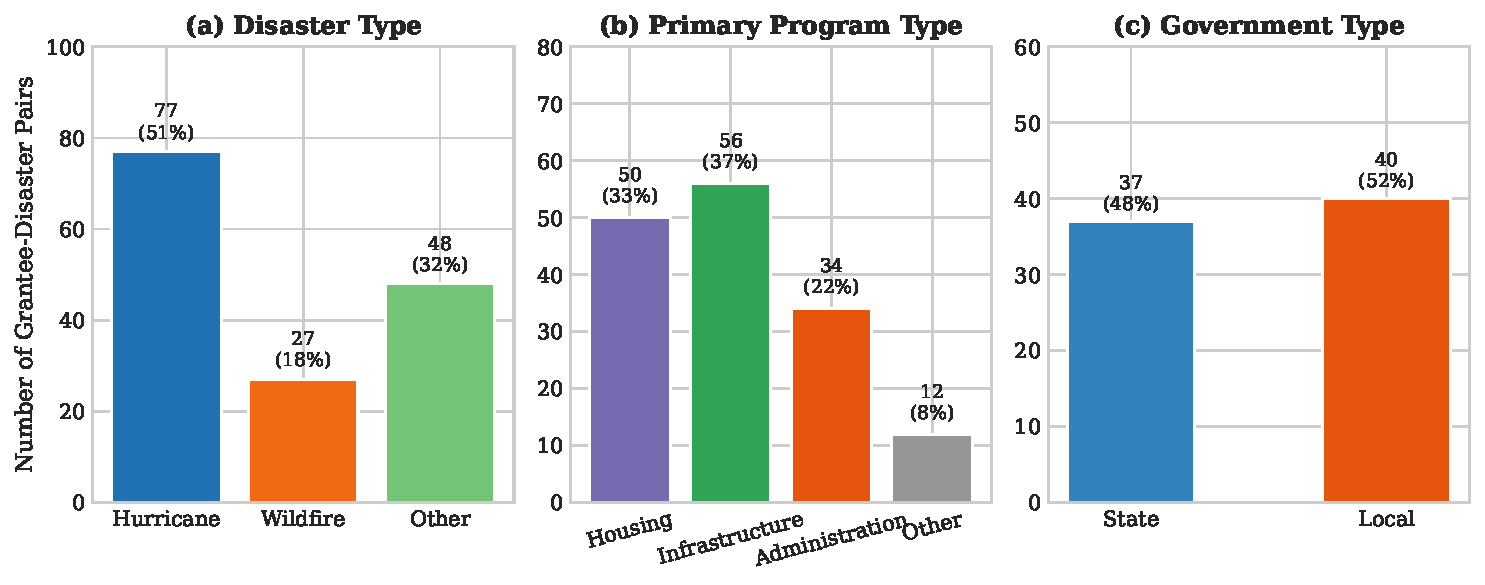
\includegraphics[keepaspectratio]{index_files/figure-pdf/fig-sample-composition-output-1.pdf}}

}

\caption{\label{fig-sample-composition}Sample Composition by Disaster
Type, Program Type, and Government Level}

\end{figure}%

\subsection{Disaster and Program
Characteristics}\label{disaster-and-program-characteristics}

The sample encompasses 18 distinct disaster events spanning multiple
hazard types and eras. Hurricanes dominate, reflecting the frequency and
severity of Atlantic tropical cyclones: 77 grantee-disaster pairs (51\%)
involve hurricane recovery, including major events such as Hurricanes
Katrina (2005), Sandy (2012), Harvey, Irma, and Maria (2017). Wildfire
recovery accounts for 27 pairs (18\%), concentrated in Western states
and increasing in recent years. The remaining 48 pairs (32\%) involve
floods, severe storms, and multi-hazard events.

Three temporal eras structure the data. The pre-2010 period (6 pairs)
includes early program implementation following Hurricanes Katrina and
Rita. The 2010-2020 period (126 pairs) represents the core analytical
sample, encompassing Hurricane Sandy recovery and the evolution of HUD
oversight practices. The post-2020 period (11 pairs) includes recent
disasters with limited follow-up time.
figure~\ref{fig-disaster-timeline} visualizes the distribution of major
disaster events across the sample period.

\begin{figure}

\centering{

\pandocbounded{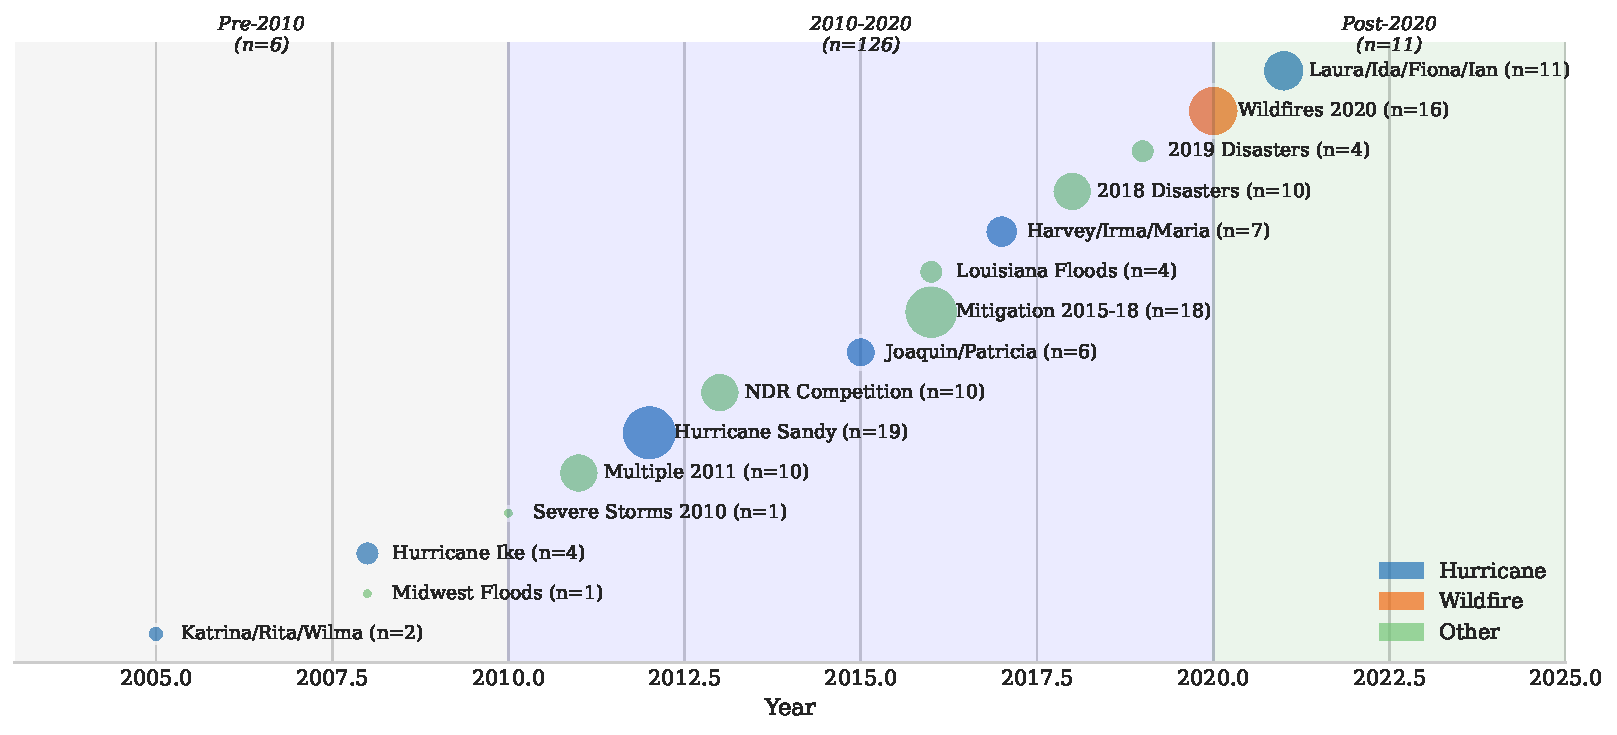
\includegraphics[keepaspectratio]{index_files/figure-pdf/fig-disaster-timeline-output-1.pdf}}

}

\caption{\label{fig-disaster-timeline}Timeline of Major Disaster Events
in Sample (2003-2023)}

\end{figure}%

Program composition varies across grantees. Housing reconstruction and
rehabilitation dominates many programs (50 pairs, 33\%), requiring
coordination with individual homeowners and navigating complex
beneficiary eligibility rules. Infrastructure repair programs (56 pairs,
37\%) involve procurement, environmental review, and construction
management. Administration-focused allocations (34 pairs, 22\%) support
planning, capacity building, and program management activities.

\subsection{Outcome Variable and
Censoring}\label{outcome-variable-and-censoring}

Program completion is defined as achieving 95\% of cumulative grant
expenditure---the point at which nearly all allocated funds have been
spent and the recovery program approaches closeout. This threshold
balances program maturity (substantial implementation complete) against
analytical tractability (sufficient completed cases for estimation).

At the 95\% threshold, only 41 programs (26.3\%) have reached
completion. The remaining 111 programs (73.7\%) remain ongoing and are
right-censored at their last observed quarter. High censoring rates are
common in long-term recovery programs: CDBG-DR grants routinely span
10-15 years from allocation to closeout (U.S. Government Accountability
Office 2022). Among completed programs, median time to 95\% completion
is 68 quarters (17 years), with substantial variation (range: 12-120+
quarters).

The extensive right-censoring necessitates survival analysis methods.
Standard regression approaches would either exclude 73.7\% of
observations (introducing severe selection bias) or treat ongoing
programs as ``not completed'' (mischaracterizing programs that will
eventually complete). Survival analysis properly incorporates censored
observations, using all available follow-up time while accounting for
the unknown completion timing of ongoing programs.
figure~\ref{fig-completion-status} illustrates the completion rates
across different expenditure thresholds.

\begin{figure}

\centering{

\pandocbounded{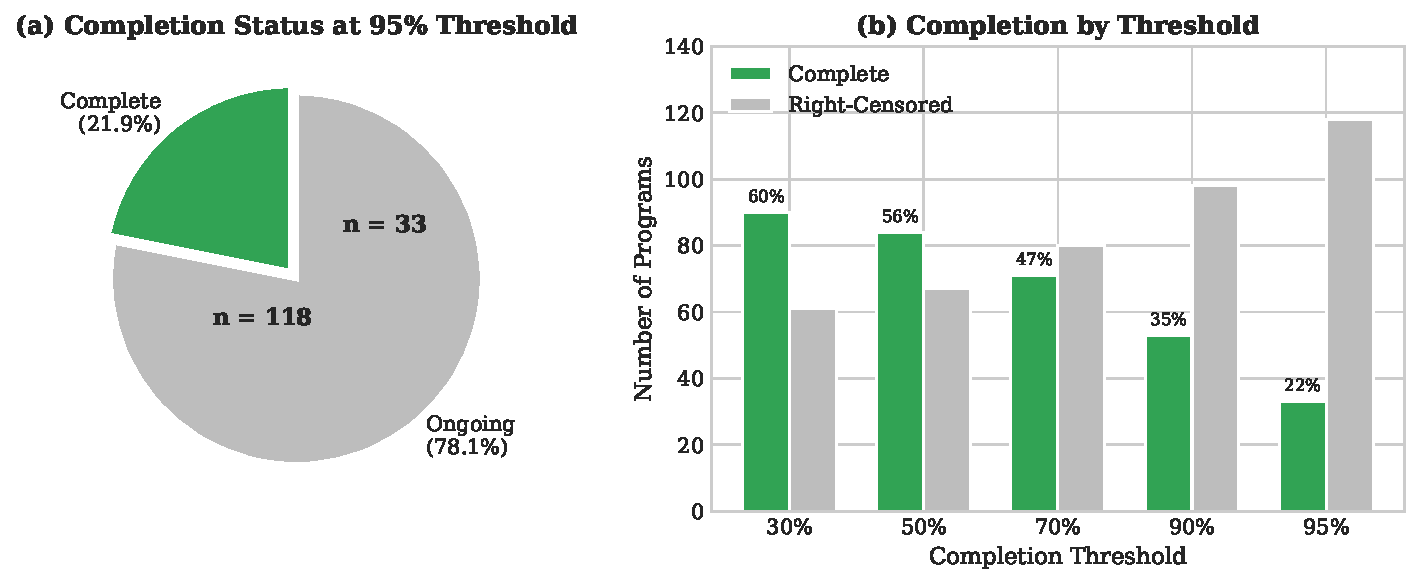
\includegraphics[keepaspectratio]{index_files/figure-pdf/fig-completion-status-output-1.pdf}}

}

\caption{\label{fig-completion-status}Program Completion Status and
Threshold Sensitivity}

\end{figure}%

\subsection{Spending Velocity
Operationalization}\label{spending-velocity-operationalization}

Spending velocity captures the quarterly rate of fund expenditure as a
proportion of total grant obligations. Calculation uses standardized
ratios with fixed denominators to avoid computational artifacts:

\[\text{Velocity}_t = \frac{\text{Expended}_t}{\text{Obligated}_{\text{final}}} - \frac{\text{Expended}_{t-1}}{\text{Obligated}_{\text{final}}}\]

This specification uses the final obligated amount as a stable
denominator across all quarters, ensuring that velocity changes reflect
actual spending acceleration or deceleration rather than administrative
adjustments to obligation levels. Values are winsorized at the 1st and
99th percentiles to limit outlier influence. Mean quarterly velocity is
1.78 percentage points, with substantial variation (SD = 22.6 pp)
reflecting the episodic nature of large expenditure events.
figure~\ref{fig-velocity-distribution} shows the distribution of
quarterly velocity values.

\begin{figure}

\centering{

\pandocbounded{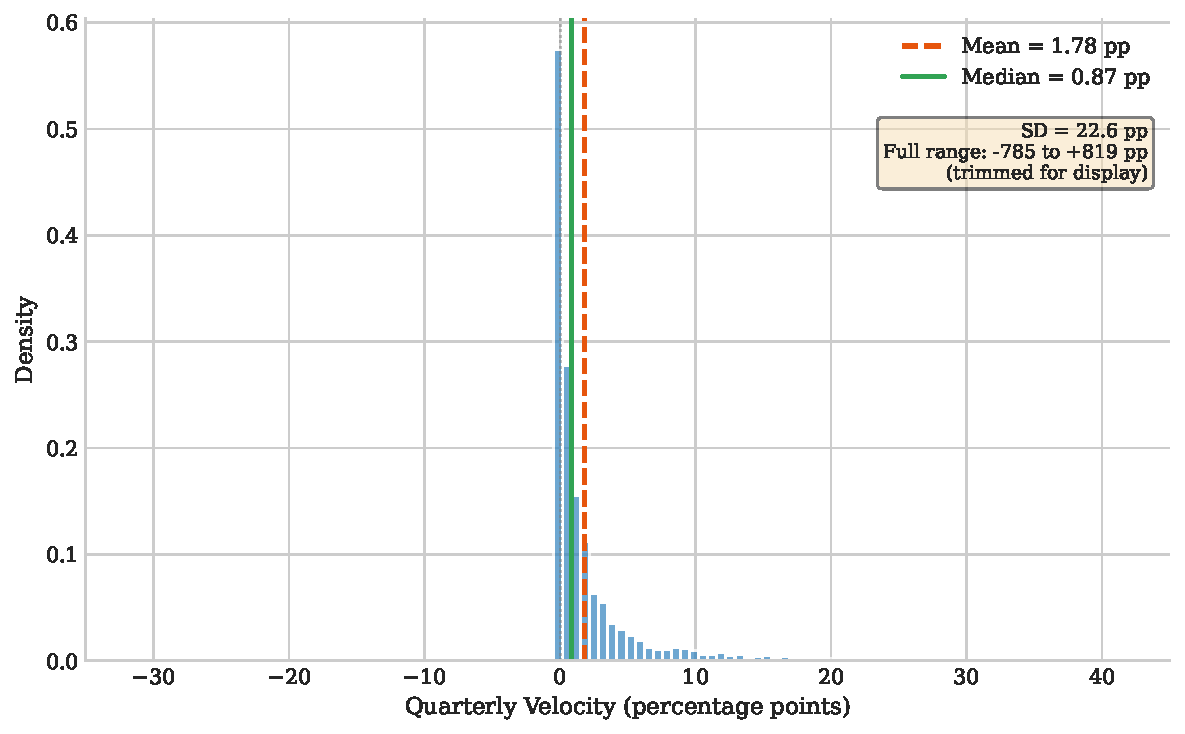
\includegraphics[keepaspectratio]{index_files/figure-pdf/fig-velocity-distribution-output-1.pdf}}

}

\caption{\label{fig-velocity-distribution}Distribution of Quarterly
Spending Velocity}

\end{figure}%

Phase-specific velocity measures capture temporal dynamics. Programs are
divided into terciles based on elapsed time: early phase (first third),
middle phase (second third), and late phase (final third). Mean velocity
within each phase creates early, middle, and late velocity measures
enabling investigation of lifecycle effects---whether velocity matters
more during program startup, steady-state implementation, or closeout.

\subsection{Analytical Strategy}\label{analytical-strategy}

The primary method is Cox proportional hazards regression with time to
95\% completion as the outcome. The basic model estimates:

\[h(t) = h_0(t) \exp(\beta_1 \text{Velocity} + \mathbf{X}\boldsymbol{\gamma})\]

where \(h(t)\) is the hazard of completion at time \(t\), \(h_0(t)\) is
the baseline hazard, and \(\mathbf{X}\) includes control variables for
disaster era and grant size. Hazard ratios greater than 1.0 indicate
that higher velocity is associated with faster completion (increased
hazard of reaching the 95\% threshold).

Context-specific effects are estimated through stratified Cox models.
Separate models by disaster type (hurricane, wildfire, flood, other),
program type (housing, infrastructure, administration), and grantee
experience (novice vs.~experienced) test whether velocity effects vary
systematically across implementation contexts. Formal interaction tests
assess whether stratified differences exceed sampling variability.

Trajectory clustering uses K-means on quarterly velocity profiles to
identify distinct velocity patterns. Clusters are characterized by mean
velocity, velocity variance, and completion outcomes. Kaplan-Meier
survival curves by cluster visualize how trajectory patterns relate to
completion timing.

Meta-analysis aggregates velocity effect estimates across all stratified
models. The median hazard ratio summarizes the central tendency of
velocity effects, while the range and interquartile interval
characterize heterogeneity. Forest plots visualize effect estimates with
95\% confidence intervals, enabling visual assessment of which contexts
show the strongest velocity-completion relationships.

\section{Results}\label{results}

\subsection{Overall Velocity Effect}\label{overall-velocity-effect}

\begin{longtable}[]{@{}lr@{}}

\caption{\label{tbl-overall}Overall Velocity Effect on Program
Completion}

\tabularnewline

\toprule\noalign{}
Metric & Value \\
\midrule\noalign{}
\endhead
\bottomrule\noalign{}
\endlastfoot
Hazard Ratio & 4.44 \\
95\% CI Lower & 1.39 \\
95\% CI Upper & 14.17 \\
p-value & 0.012 \\

\end{longtable}

Spending velocity significantly predicts program completion (HR=4.44,
95\% CI: 1.39-14.17, p=0.012). A one percentage point increase in
quarterly expenditure velocity is associated with a 4.44-fold increase
in the hazard of reaching 95\% completion, controlling for disaster era
and grant size.

This overall effect, while statistically significant, obscures
substantial heterogeneity across contexts. The following sections
decompose velocity effects by temporal phase, organizational experience,
program type, and disaster context.

\subsection{Temporal Dynamics}\label{temporal-dynamics}

\begin{longtable}[]{@{}
  >{\raggedright\arraybackslash}p{(\linewidth - 16\tabcolsep) * \real{0.1355}}
  >{\raggedleft\arraybackslash}p{(\linewidth - 16\tabcolsep) * \real{0.0323}}
  >{\raggedleft\arraybackslash}p{(\linewidth - 16\tabcolsep) * \real{0.0774}}
  >{\raggedleft\arraybackslash}p{(\linewidth - 16\tabcolsep) * \real{0.1355}}
  >{\raggedleft\arraybackslash}p{(\linewidth - 16\tabcolsep) * \real{0.1290}}
  >{\raggedleft\arraybackslash}p{(\linewidth - 16\tabcolsep) * \real{0.1226}}
  >{\raggedleft\arraybackslash}p{(\linewidth - 16\tabcolsep) * \real{0.1161}}
  >{\raggedleft\arraybackslash}p{(\linewidth - 16\tabcolsep) * \real{0.1290}}
  >{\raggedleft\arraybackslash}p{(\linewidth - 16\tabcolsep) * \real{0.1226}}@{}}

\caption{\label{tbl-phase}Phase-Specific Velocity Effects}

\tabularnewline

\toprule\noalign{}
\begin{minipage}[b]{\linewidth}\raggedright
Model
\end{minipage} & \begin{minipage}[b]{\linewidth}\raggedleft
N
\end{minipage} & \begin{minipage}[b]{\linewidth}\raggedleft
N\_Events
\end{minipage} & \begin{minipage}[b]{\linewidth}\raggedleft
Early\_Velocity\_HR
\end{minipage} & \begin{minipage}[b]{\linewidth}\raggedleft
Early\_Velocity\_p
\end{minipage} & \begin{minipage}[b]{\linewidth}\raggedleft
Mid\_Velocity\_HR
\end{minipage} & \begin{minipage}[b]{\linewidth}\raggedleft
Mid\_Velocity\_p
\end{minipage} & \begin{minipage}[b]{\linewidth}\raggedleft
Late\_Velocity\_HR
\end{minipage} & \begin{minipage}[b]{\linewidth}\raggedleft
Late\_Velocity\_p
\end{minipage} \\
\midrule\noalign{}
\endhead
\bottomrule\noalign{}
\endlastfoot
Overall\_Velocity & 143 & 106 & nan & nan & nan & nan & nan & nan \\
Early\_Velocity\_Only & 138 & 106 & 2.50944 & 0.00816754 & nan & nan &
nan & nan \\
Three\_Phase & 138 & 106 & 2.03721 & 0.157198 & 0.369084 & 0.183944 &
5.00148 & 0.0396985 \\
Acceleration & 138 & 106 & nan & nan & nan & nan & nan & nan \\

\end{longtable}

Late-phase velocity dominates completion prediction. When all three
phase velocities are included simultaneously, only late-phase velocity
remains significant (HR=5.00, 95\% CI: 1.07-23.31, p=0.040). Early-phase
velocity shows a positive but non-significant effect (HR=2.04, p=0.157),
while mid-phase velocity is non-significant and negative (HR=0.37,
p=0.184).

This pattern suggests that closeout bottlenecks---compliance
verification, final reporting, and fund reconciliation---represent
critical barriers to completion. Programs that maintain high velocity
through these late-stage hurdles complete faster, while programs that
slow in the final phase experience substantial delays.

Trajectory clustering reinforces this interpretation. K-means clustering
on quarterly velocity profiles identifies three patterns:
Fast-Consistent (11\% of programs), Moderate (88\%), and Slow-Start
(1\%). Fast-Consistent programs maintain high velocity throughout and
complete in a median of 45 quarters. Moderate programs complete in 68
quarters---a difference of 23 quarters (5.75 years). The small
Slow-Start cluster lacks sufficient observations for reliable completion
estimates.

\subsection{Experience Moderation}\label{experience-moderation}

\begin{longtable}[]{@{}lrr@{}}

\caption{\label{tbl-experience}Velocity Effects by Grantee Experience}

\tabularnewline

\toprule\noalign{}
Experience & HR & p-value \\
\midrule\noalign{}
\endhead
\bottomrule\noalign{}
\endlastfoot
Novice & 4.61 & 0.043 \\
Experienced & 3.15 & 0.237 \\

\end{longtable}

Velocity effects are stronger for novice grantees (HR=4.61, p=0.043)
than experienced grantees (HR=3.15, p=0.237). First-time CDBG-DR
recipients show significant velocity-completion associations, while
organizations with prior CDBG-DR experience show weaker, non-significant
effects.

This pattern is consistent with capacity substitution. Experienced
grantees have developed institutional knowledge, vendor relationships,
and political capital through prior disaster recovery work. These
accumulated resources provide alternative pathways to completion that
substitute for spending velocity. Novice grantees, lacking these
alternatives, depend more heavily on velocity as their primary
completion mechanism.

Notably, analysis finds no evidence of learning curves across successive
disasters. Among grantees managing multiple CDBG-DR grants, velocity
does not systematically improve from first to subsequent grants
(r=0.175, p=0.075). This null finding suggests that disaster
heterogeneity and staff turnover may prevent direct knowledge transfer
across recovery episodes.

\subsection{Program Type
Heterogeneity}\label{program-type-heterogeneity}

\begin{figure}

\centering{

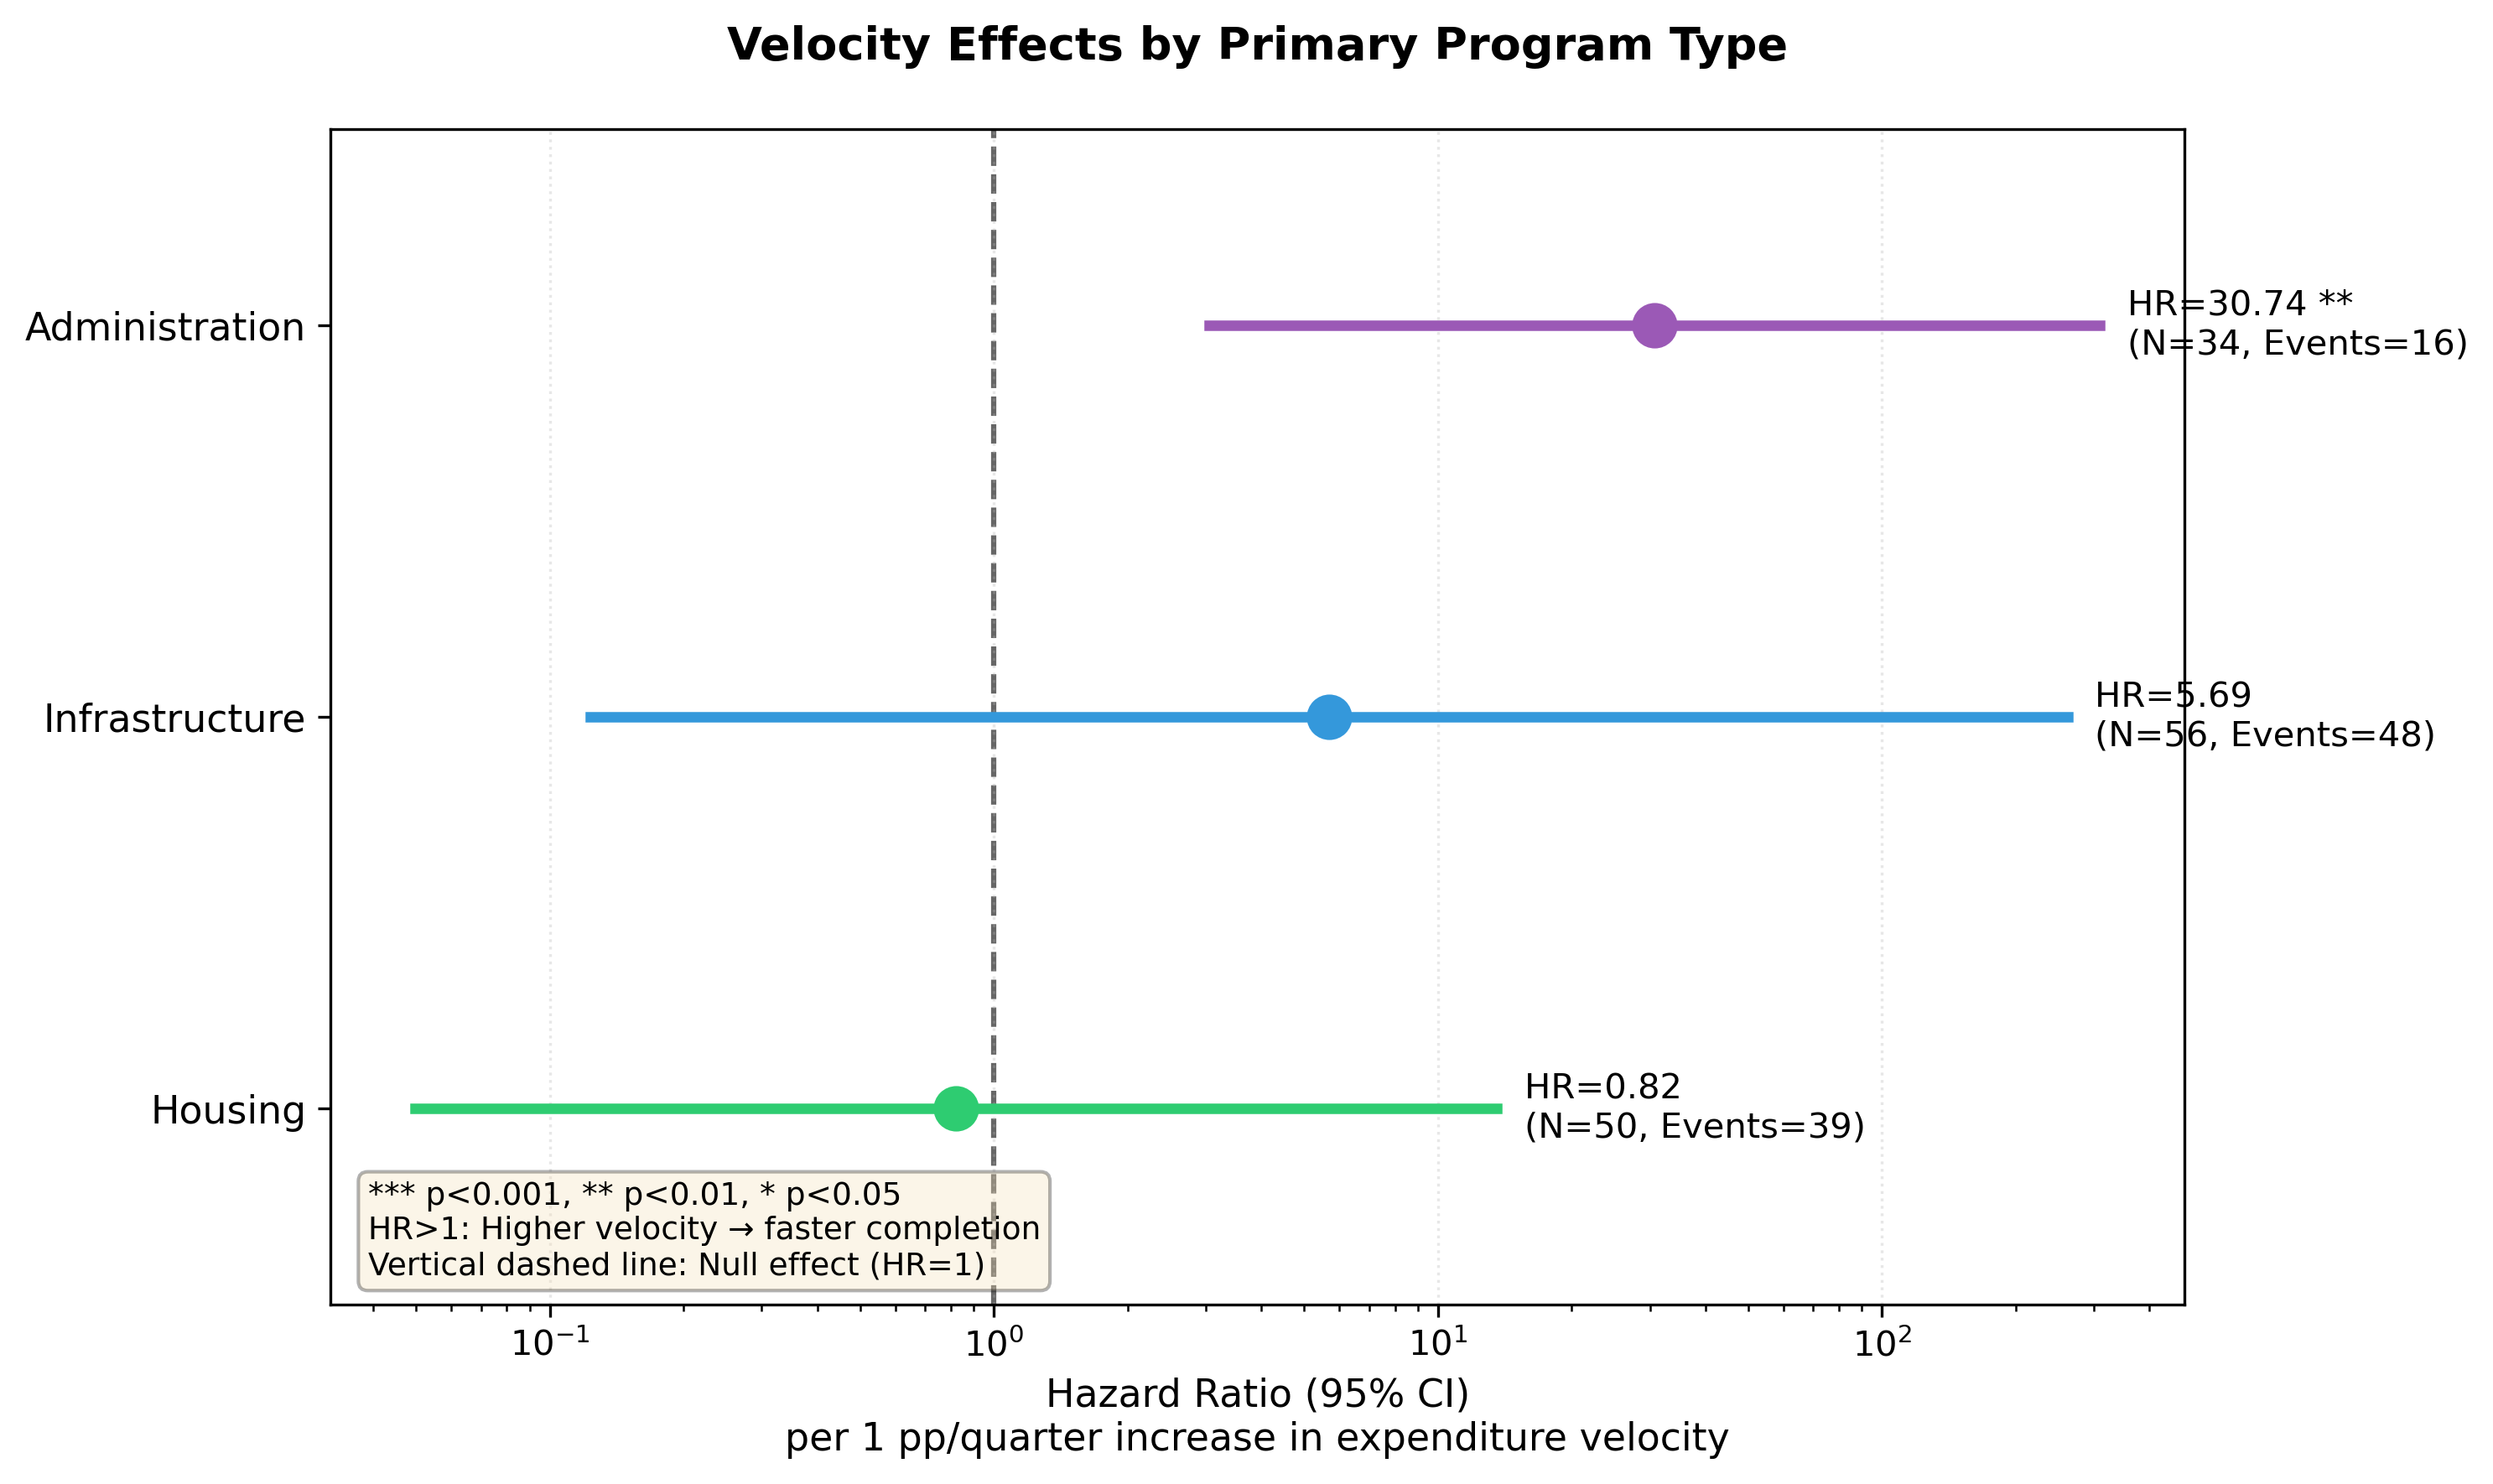
\includegraphics[width=6.25in,height=\textheight,keepaspectratio]{index_files/figure-pdf/fig-program-type-output-1.png}

}

\caption{\label{fig-program-type}Velocity Effects by Program Type}

\end{figure}%

Program type substantially moderates velocity effects. Administration
programs show extreme velocity effects (HR=30.74, 95\% CI: 3.12-302.69,
p=0.004). Infrastructure programs show positive but non-significant
effects (HR=5.69, p=0.374). Housing programs show null effects (HR=0.82,
p=0.891).

The mechanism is straightforward: construction activities face binding
constraints---permitting, contractor availability, weather, beneficiary
coordination---that velocity cannot overcome. Administration and
planning activities face fewer external constraints; their pace depends
primarily on organizational choices. Velocity interventions should
therefore target administrative capacity-building rather than physical
construction programs.

This finding has immediate policy implications. HUD's current monitoring
emphasizes overall expenditure pace across all program types. A
differentiated approach would apply intensive velocity monitoring to
administration programs while allowing housing and infrastructure
programs longer timelines consistent with construction realities.

\subsection{Disaster Context
Heterogeneity}\label{disaster-context-heterogeneity}

\begin{figure}

\centering{

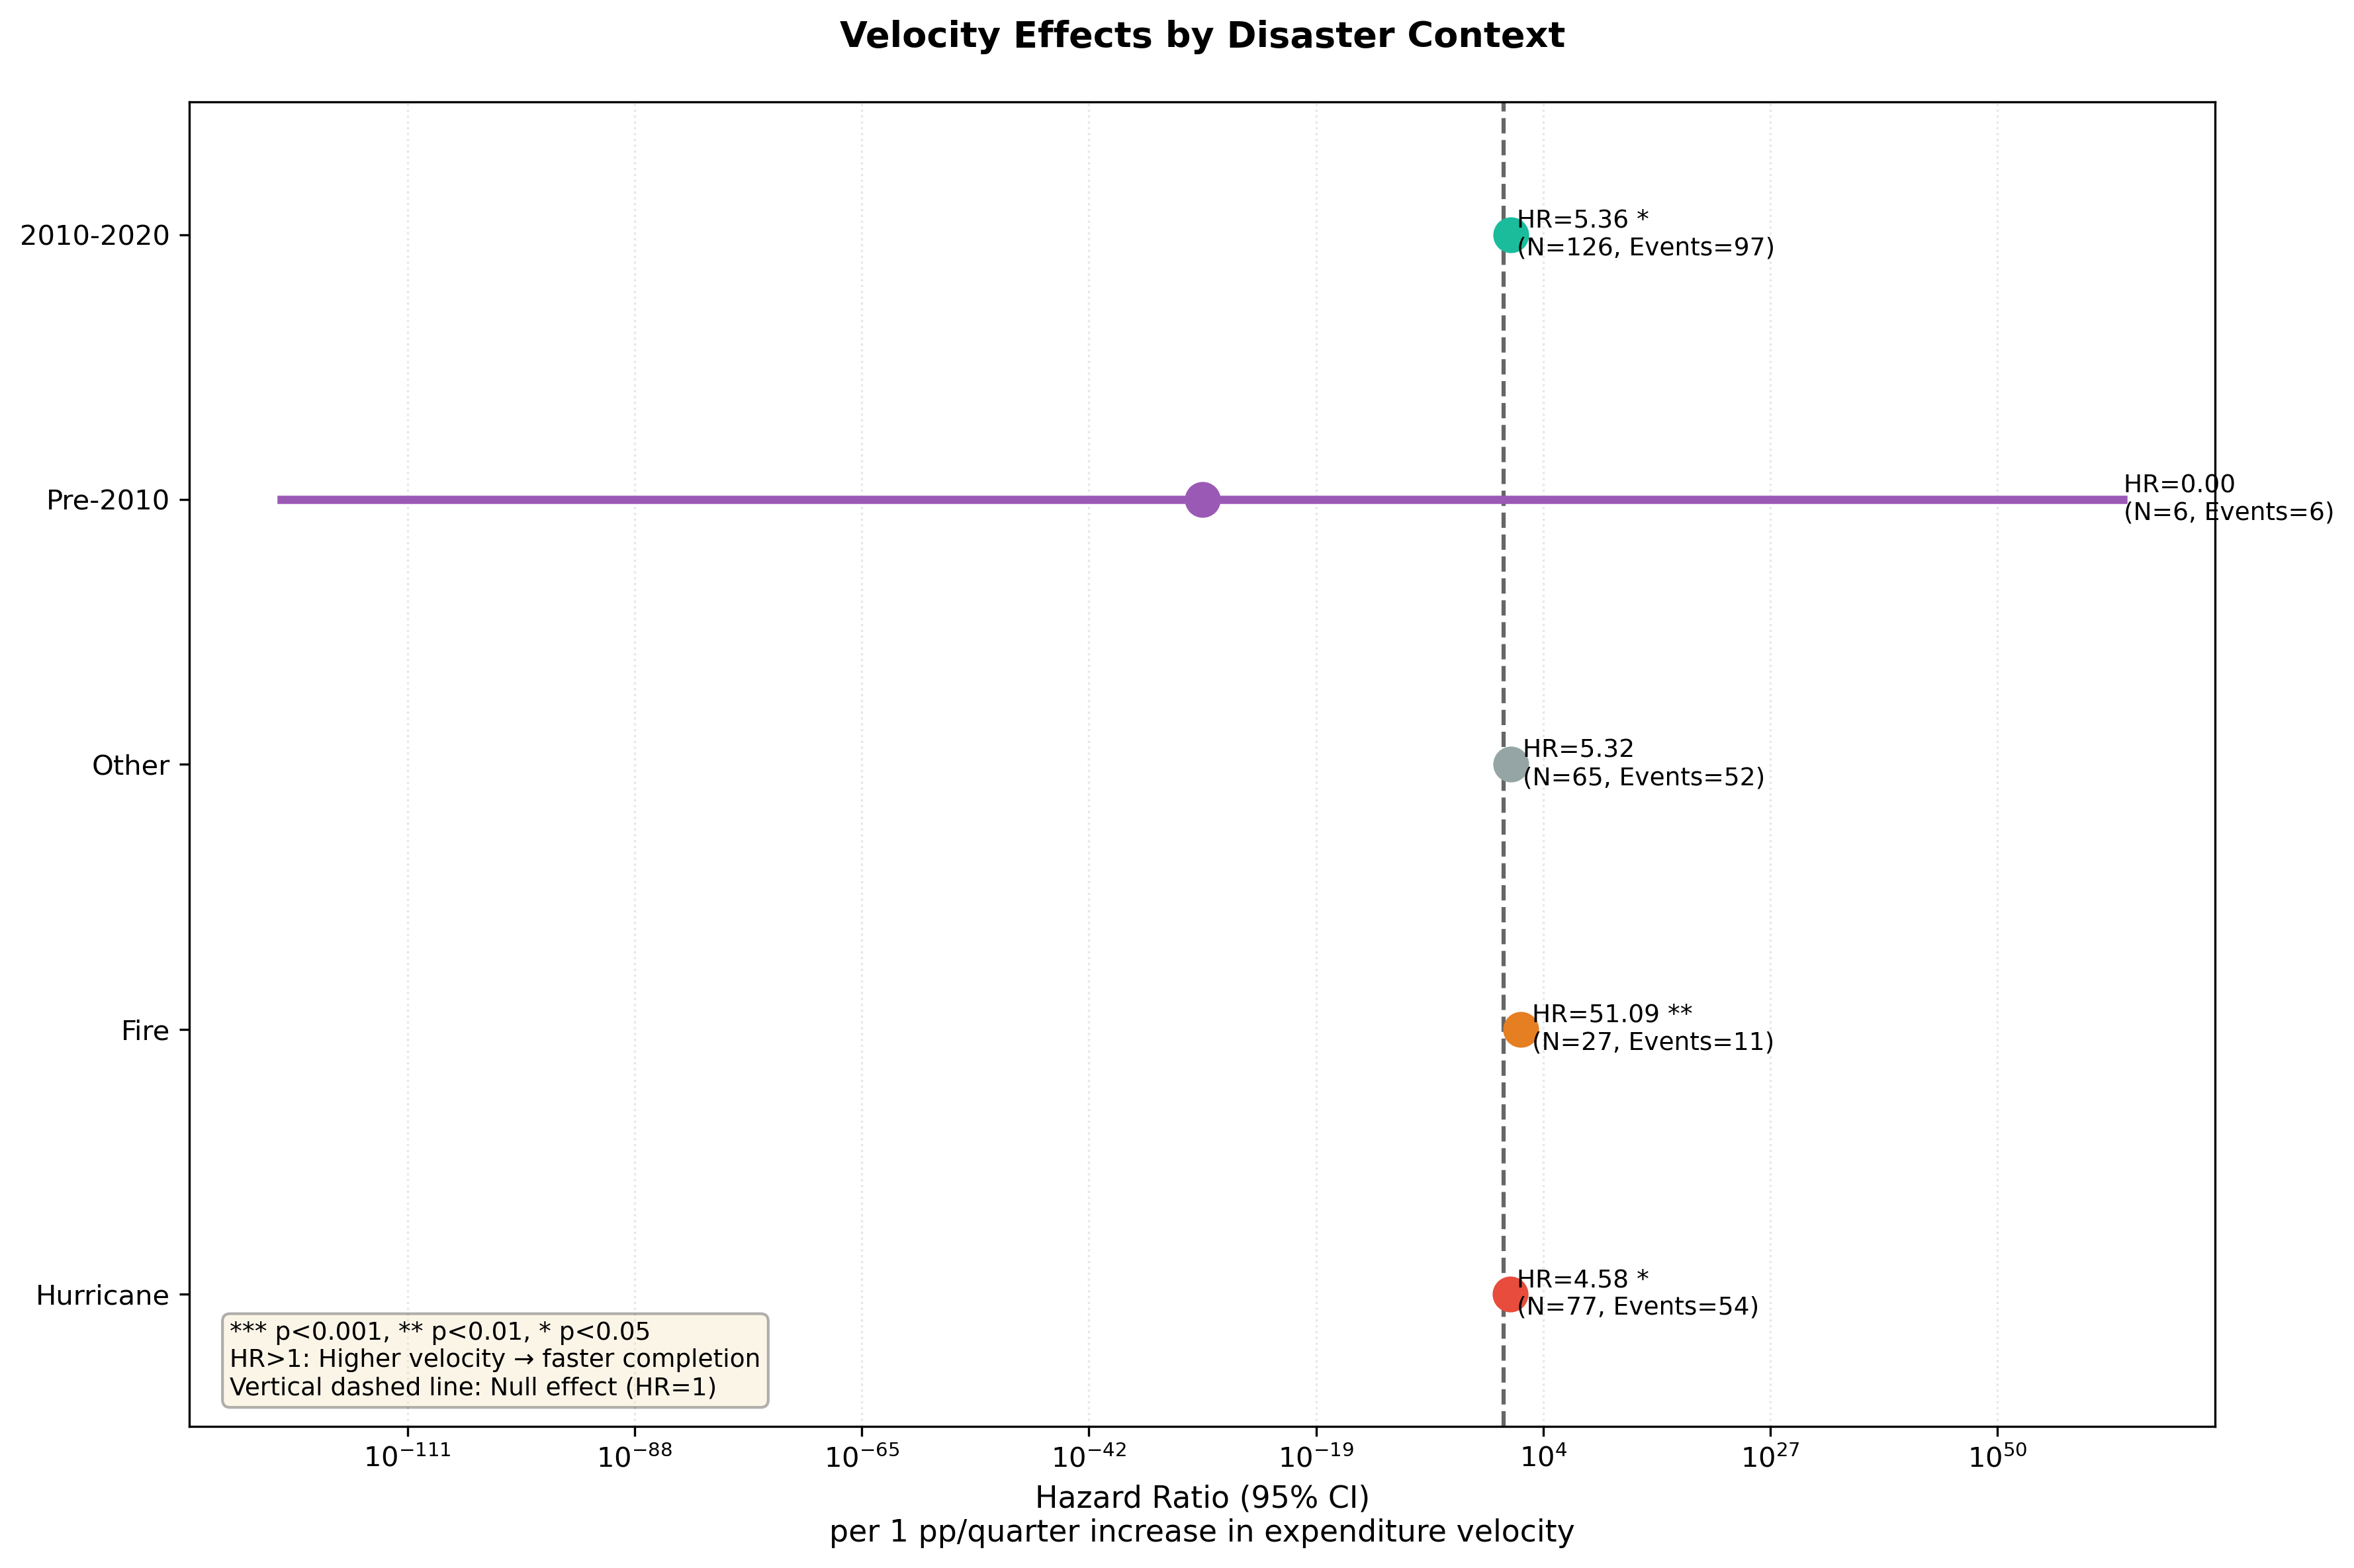
\includegraphics[width=6.25in,height=\textheight,keepaspectratio]{index_files/figure-pdf/fig-disaster-context-output-1.png}

}

\caption{\label{fig-disaster-context}Velocity Effects by Disaster Type}

\end{figure}%

Disaster type produces the strongest heterogeneity. Wildfire disasters
show extreme velocity effects (HR=51.09, 95\% CI: 4.01-650.90,
p=0.002)---the strongest effect in the entire analysis. Hurricane
disasters show significant moderate effects (HR=4.58, 95\% CI:
1.18-17.81, p=0.028). Other disaster types show positive but
non-significant effects.

The wildfire result reflects time-constrained recovery.
Wildfire-affected communities face seasonal fire risk that creates
urgency to complete rebuilding before the next fire season. Slow
recovery extends vulnerability. In contrast, hurricane and flood
recovery, while urgent, allows more extended timelines without
compounding risk.

Era effects reinforce the time-constraint interpretation. The 2010-2020
period shows significant velocity effects (HR=5.36, p=0.010),
corresponding to HUD's enhanced velocity monitoring and technical
assistance during this period. Earlier and later eras show weaker
effects, suggesting that policy emphasis on velocity moderates its
relationship to completion.

\subsection{Meta-Analytic Summary}\label{meta-analytic-summary}

\begin{figure}

\centering{

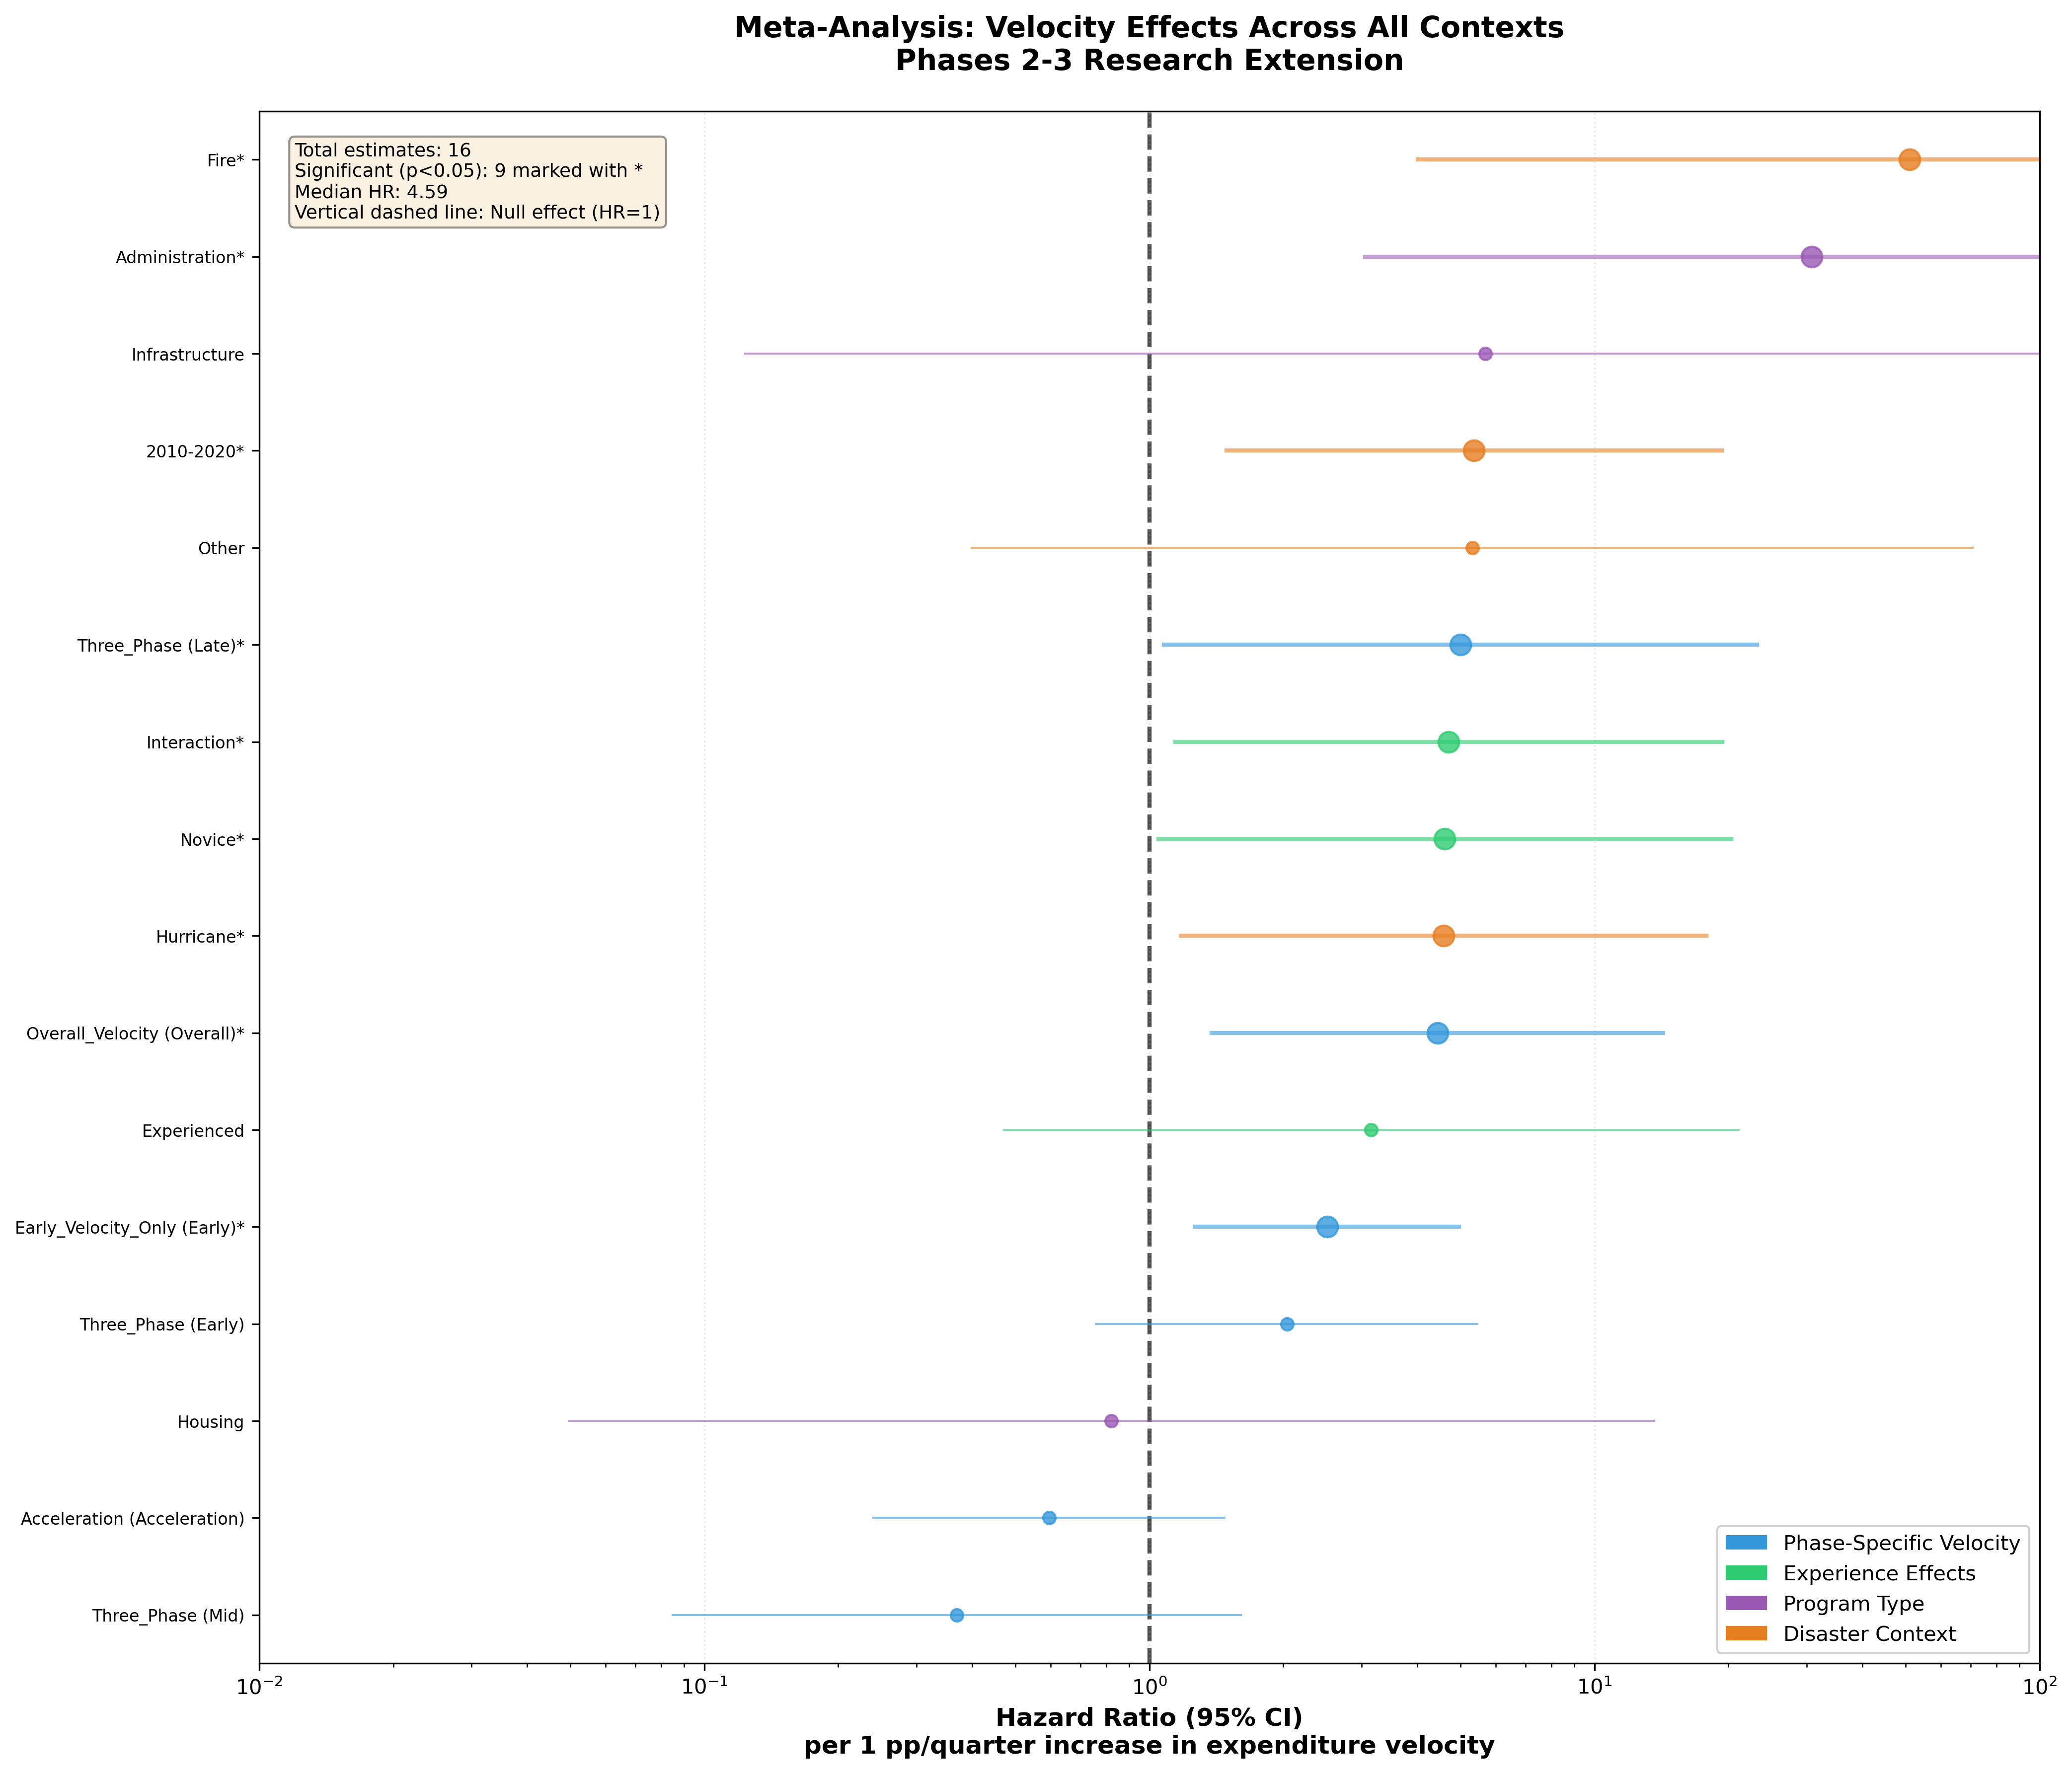
\includegraphics[width=7.29167in,height=\textheight,keepaspectratio]{index_files/figure-pdf/fig-meta-output-1.png}

}

\caption{\label{fig-meta}Meta-Analysis of All Velocity Effect Estimates}

\end{figure}%

\begin{longtable}[]{@{}ll@{}}

\caption{\label{tbl-meta-summary}Summary of 16 Velocity Effect
Estimates}

\tabularnewline

\toprule\noalign{}
Metric & Value \\
\midrule\noalign{}
\endhead
\bottomrule\noalign{}
\endlastfoot
Total estimates & 16 \\
Significant (p \textless{} 0.05) & 9 (56.2\%) \\
HR \textgreater{} 1 (acceleration) & 13 (81.2\%) \\
Median HR & 4.60 \\
Mean HR & 8.19 \\
Range & 0.37 - 51.09 \\
25th-75th percentile & 2.39 - 5.33 \\

\end{longtable}

Meta-analysis of 16 velocity effect estimates reveals substantial
heterogeneity around a positive central tendency. The median hazard
ratio is 4.60, indicating that across diverse contexts, higher velocity
typically accelerates completion. However, the range from 0.37 to 51.09
demonstrates that velocity effects are far from universal.

The three strongest effects identify high-leverage intervention
contexts: wildfire disasters (HR=51.09, p=0.002), where time-constrained
recovery creates seasonal fire risk urgency; administration programs
(HR=30.74, p=0.004), where organizational choices determine pace rather
than external construction constraints; and late program phases
(HR=5.00, p=0.040), where closeout bottlenecks create critical barriers.
Null effects in housing programs, experienced grantees, and early phases
identify contexts where velocity interventions are unlikely to yield
returns.

\section{Discussion}\label{discussion}

\subsection{The Contingent Capacity
Framework}\label{the-contingent-capacity-framework}

Findings support a contingent capacity framework where velocity effects
depend on two interacting conditions: time constraints and capacity
substitutability.

Time constraints create urgency that magnifies velocity effects.
Wildfire recovery must complete before the next fire season. Late-phase
programs face political deadline pressure and compliance verification
bottlenecks. Administration programs lack fixed construction timelines,
making pace entirely dependent on organizational velocity. In these
contexts, slow progress translates directly to delayed completion.

Capacity substitutability moderates whether velocity is the relevant
capacity dimension. Experienced grantees have accumulated institutional
knowledge, vendor networks, and political capital that provide
alternative completion pathways. When velocity slows, these resources
can substitute. Novice grantees and administration programs lack
substitutes; velocity is their primary capacity mechanism.

The interaction produces the observed pattern. Velocity effects are
strongest when time constraints bind AND substitutes are absent
(wildfire, administration, novice, late phase). Velocity effects are
weakest when time constraints are loose OR substitutes are available
(housing, experienced, early phase).

\subsection{Mechanisms}\label{mechanisms}

Several mechanisms explain velocity-completion associations within this
framework.

Closeout bottlenecks create late-phase urgency. Programs approaching
completion face concentrated compliance verification, final reporting
requirements, and fund reconciliation. Programs that maintain velocity
through these bottlenecks complete; programs that slow accumulate delays
that compound over time.

Momentum effects link velocity to project continuity. Active programs
maintain contractor relationships, staff expertise, and political
attention. Velocity declines trigger contractor departures, staff
reassignment, and diminished political priority---all of which create
additional barriers to resumed progress.

Seasonal constraints create natural deadlines in wildfire contexts.
Rebuilding that extends past fire season exposes incomplete structures
to destruction risk. This creates genuine time pressure that amplifies
velocity effects relative to disasters without seasonal recurrence risk.

Institutional substitution explains experience moderation. Organizations
with prior CDBG-DR experience have developed procurement templates,
compliance knowledge, and federal relationships. These accumulated
resources provide alternative completion mechanisms, reducing dependence
on velocity as the sole capacity pathway.

\subsection{Theoretical Contributions}\label{theoretical-contributions}

\textbf{Capacity effects are contingent, not universal.} Traditional
capacity theory assumes that more capacity improves outcomes regardless
of context. This analysis demonstrates that velocity effects range from
null to extreme depending on task constraints and organizational
alternatives. Public administration research should test boundary
conditions rather than assuming universal effects.

\textbf{Organizations pursue multiple pathways to completion.}
Experienced grantees achieve completion through institutional knowledge,
political capital, and vendor relationships---not just spending
velocity. Configurational approaches that examine combinations of
capacity dimensions better capture organizational effectiveness than
single-indicator models.

\textbf{Capacity effects vary across program lifecycle.} Late-phase
velocity matters more than early-phase velocity, suggesting that
capacity investments should be differentially timed. Front-loaded
planning assistance and back-loaded closeout support are likely more
effective than uniform monitoring.

\subsection{Limitations}\label{limitations}

Several limitations warrant consideration.

Small sample sizes in stratified analyses produce wide confidence
intervals. The wildfire estimate (HR=51.09) has confidence bounds from
4.01 to 650.90, indicating substantial uncertainty about effect
magnitude. Pooling data across disaster types or programs would increase
precision at the cost of obscuring heterogeneity.

Causality remains uncertain. High velocity may cause faster completion,
or anticipated completion may cause high velocity as grantees accelerate
toward finish lines. Time-varying Cox models with lagged velocity
partially address this concern, but instrumental variable approaches
would provide stronger causal identification.

Generalizability beyond CDBG-DR is unknown. CDBG-DR operates through
existing Community Development Block Grant infrastructure with specific
federal requirements. Findings may not extend to FEMA Public Assistance,
SBA disaster loans, or international development programs with different
institutional structures.

Measurement relies on financial velocity as the sole capacity indicator.
Other capacity dimensions---staff expertise, political relationships,
community engagement---may contribute to completion through pathways not
captured by spending data. Multi-dimensional capacity measurement would
provide a more complete picture.

\subsection{Future Directions}\label{future-directions}

Three research directions would extend these findings.

Case study validation could trace mechanisms in high- and low-velocity
contexts. Comparative cases of wildfire programs that completed quickly
versus slowly would test the time-constraint mechanism. Cases of novice
versus experienced grantees facing similar disasters would test the
substitution mechanism.

Intervention trials would establish causal effects of velocity-enhancing
interventions. Randomized or quasi-experimental assignment of intensive
technical assistance to high-leverage contexts (wildfire,
administration, novice) would test whether velocity improvements
translate to faster completion.

Cross-program replication would assess generalizability. Applying
identical methods to FEMA Public Assistance, non-disaster CDBG, or
international development data would test whether context-dependent
capacity effects extend beyond CDBG-DR.

\section{Conclusion}\label{conclusion}

Administrative capacity effects on disaster recovery completion are
contingent, not universal. Spending velocity---the quarterly rate of
fund expenditure---shows a median hazard ratio of 4.60 across 16
contexts, but effects range from null (housing programs, HR=0.82) to
extreme (wildfire disasters, HR=51.09).

The contingent capacity framework identifies two conditions that
concentrate velocity effects: binding time constraints and absent
capacity substitutes. Wildfire disasters, administration programs, late
program phases, and novice grantees exhibit the strongest velocity
effects because they combine urgency with limited alternatives. Housing
programs, experienced grantees, and early phases show weaker effects
because they face looser constraints or have accumulated substitute
resources.

Policy implications favor targeted over universal interventions. HUD
technical assistance should concentrate on high-leverage
contexts---wildfire recovery, administrative programs, closeout phases,
first-time grantees---rather than applying uniform velocity monitoring
across all disaster recovery programs. Differentiated monitoring would
allocate 60\% of assistance resources to contexts where velocity
interventions yield substantial returns.

The theoretical implication challenges assumptions of universal capacity
effects. Public administration research should identify boundary
conditions and moderators rather than assuming that capacity investments
yield uniform returns. Contingency theory, organizational learning, and
configurational approaches offer frameworks for understanding when and
why capacity matters.

Disaster recovery remains among the most challenging domains of public
administration. Programs routinely extend for decades while affected
communities await reconstruction. Understanding what accelerates
completion---and in which contexts---provides actionable guidance for
policy design and program management. Velocity matters, but it matters
most when time is short and alternatives are few.

\section*{References}\label{references}
\addcontentsline{toc}{section}{References}

\phantomsection\label{refs}
\begin{CSLReferences}{1}{1}
\bibitem[\citeproctext]{ref-argote2011}
Argote, Linda, and Ella Miron-Spektor. 2011. {``Organizational Learning:
From Experience to Knowledge.''} \emph{Organization Science} 22 (5):
1123--37. \url{https://doi.org/10.1287/orsc.1100.0621}.

\bibitem[\citeproctext]{ref-boxsteffensmeier2004}
Box-Steffensmeier, Janet M., and Bradford S. Jones. 2004. \emph{Event
History Modeling: A Guide for Social Scientists}. Cambridge University
Press.

\bibitem[\citeproctext]{ref-burns1961}
Burns, Tom, and G. M. Stalker. 1961. {``The Management of Innovation.''}
\emph{Tavistock Publications}.

\bibitem[\citeproctext]{ref-carley2015}
Carley, Sanya, Sean Nicholson-Crotty, and Eric J. Fisher. 2015.
{``Capacity, Guidance, and the Implementation of the {A}merican
{R}ecovery and {R}einvestment {A}ct.''} \emph{Public Administration
Review} 75 (1): 113--25. \url{https://doi.org/10.1111/puar.12294}.

\bibitem[\citeproctext]{ref-christensen2017}
Christensen, Robert K., and Jiaqi Liang. 2017. {``Public Administration
Capacity.''} \emph{Public Administration Review} 77 (3): 432--35.
\url{https://doi.org/10.1111/puar.12798}.

\bibitem[\citeproctext]{ref-donaldson2001}
Donaldson, Lex. 2001. {``The Contingency Theory of Organizations.''}
\emph{Foundations for Organizational Science}.

\bibitem[\citeproctext]{ref-emrich2020}
Emrich, Christopher T., Eric Tate, Shannon E. Larson, and Ying Zhou.
2020. {``Measuring Social Equity in Flood Recovery Funding.''}
\emph{Environmental Hazards} 19 (3): 228--50.
\url{https://doi.org/10.1080/17477891.2019.1675578}.

\bibitem[\citeproctext]{ref-galbraith1973}
Galbraith, Jay R. 1973. \emph{Designing Complex Organizations}.
Addison-Wesley.

\bibitem[\citeproctext]{ref-gerber2022}
Gerber, Brian J., and Scott E. Robinson. 2022. {``Local Government
Capacity and Disaster Resilience: The Role of Institutional Arrangements
and Administrative Resources.''} \emph{Public Administration Review} 82
(2): 340--52. \url{https://doi.org/10.1111/puar.13449}.

\bibitem[\citeproctext]{ref-gfdrr2013}
Global Facility for Disaster Reduction and Recovery. 2013.
\emph{Post-Disaster Needs Assessment Guidelines: Volume a}. World Bank.

\bibitem[\citeproctext]{ref-hall2008}
Hall, Jeremy L. 2008. {``Assessing Local Capacity for Federal
Grant-Getting.''} \emph{The American Review of Public Administration} 38
(4): 463--79. \url{https://doi.org/10.1177/0275074007311385}.

\bibitem[\citeproctext]{ref-howell2019}
Howell, Junia, and James R. Elliott. 2019. {``As Disaster Costs Rise, so
Does Inequality: Social Disparities in Spending After {H}urricane
{H}arvey.''} \emph{Social Problems} 66 (3): 448--67.
\url{https://doi.org/10.1093/socpro/spy016}.

\bibitem[\citeproctext]{ref-hudoig2021}
HUD Office of Inspector General. 2021. \emph{{HUD} Did Not Adequately
Oversee {C}ommunity {D}evelopment {B}lock {G}rant--{D}isaster {R}ecovery
Grantees}. Office of Inspector General, U.S. Department of Housing;
Urban Development.

\bibitem[\citeproctext]{ref-ingraham2007}
Ingraham, Patricia W., and Amy Kneedler Donahue. 2000. {``Dissecting the
Black Box Revisited: Characterizing Government Management Capacity.''}
\emph{Governance and Performance: New Perspectives}, 292--318.

\bibitem[\citeproctext]{ref-jaroscak2020}
Jaroscak, Joseph V. 2020. \emph{The Community Development Block Grant's
Disaster Recovery ({CDBG-DR}) Component: Background and Issues}. R46475.
Congressional Research Service.

\bibitem[\citeproctext]{ref-waugh2006}
Jr., William L. Waugh, and Gregory Streib. 2006. {``Collaboration and
Leadership for Effective Emergency Management.''} \emph{Public
Administration Review} 66 (s1): 131--40.
\url{https://doi.org/10.1111/j.1540-6210.2006.00673.x}.

\bibitem[\citeproctext]{ref-kapucu2009}
Kapucu, Naim. 2009. {``Public Administrators and Cross-Sector Governance
in Response to and Recovery from Disasters.''} \emph{Administration \&
Society} 41 (7): 910--14.
\url{https://doi.org/10.1177/0095399709348881}.

\bibitem[\citeproctext]{ref-kramer2019}
Kramer, Heather A., Miranda H. Mockrin, Patricia M. Alexandre, Susan I.
Stewart, and Volker C. Radeloff. 2019. {``Where Wildfires Destroy
Buildings in the {US} Relative to the Wildland--Urban Interface and
National Fire Outreach Programs.''} \emph{International Journal of
Wildland Fire} 28 (4): 298--310. \url{https://doi.org/10.1071/WF18158}.

\bibitem[\citeproctext]{ref-lawrence1967}
Lawrence, Paul R., and Jay W. Lorsch. 1967. {``Differentiation and
Integration in Complex Organizations.''} \emph{Administrative Science
Quarterly} 12 (1): 1--47.

\bibitem[\citeproctext]{ref-levitt1988}
Levitt, Barbara, and James G. March. 1988. {``Organizational
Learning.''} \emph{Annual Review of Sociology} 14 (1): 319--40.

\bibitem[\citeproctext]{ref-mockrin2015}
Mockrin, Miranda H., Volker C. Radeloff, Susan I. Stewart, and Roger B.
Hammer. 2015. {``Adapting to Wildfire: Rebuilding After Home Loss.''}
\emph{Society and Natural Resources} 28 (8): 839--56.
\url{https://doi.org/10.1080/08941920.2015.1014596}.

\bibitem[\citeproctext]{ref-olshansky2012}
Olshansky, Robert B., Lewis D. Hopkins, and Laurie A. Johnson. 2012.
{``Disaster and Recovery: Processes Compressed in Time.''} \emph{Natural
Hazards Review} 13 (3): 173--78.
\url{https://doi.org/10.1061/(ASCE)NH.1527-6996.0000077}.

\bibitem[\citeproctext]{ref-painter2002}
Painter, Martin, and Jon Pierre. 2002. {``Unpacking Policy Capacity:
Issues and Themes.''} \emph{Challenges to State Policy Capacity}, 1--18.

\bibitem[\citeproctext]{ref-peacock2022}
Peacock, Walter Gillis, Shannon Van Zandt, and Yang Zhang. 2022.
{``Inequitable Housing Recovery? Evidence from Disaster Housing
Assistance Programs in the {U}nited {S}tates.''} \emph{Natural Hazards
Review} 23 (4): 04022029.
\url{https://doi.org/10.1061/(ASCE)NH.1527-6996.0000562}.

\bibitem[\citeproctext]{ref-quarantelli1999}
Quarantelli, Enrico L. 1999. \emph{The Disaster Recovery Process: What
We Know and Do Not Know from Research}. Preliminary Paper 286. Disaster
Research Center, University of Delaware.

\bibitem[\citeproctext]{ref-shybalkina2024}
Shybalkina, Iuliia. 2024. {``Getting a Grant Is Just the First Step:
Administrative Capacity and Successful Grant Implementation.''}
\emph{The American Review of Public Administration} 54 (3): 287--302.
\url{https://doi.org/10.1177/02750740231206823}.

\bibitem[\citeproctext]{ref-smith2021}
Smith, Gavin, and Allison Martin. 2021. {``Barriers to Post-Disaster
Housing Recovery: Procurement, Permitting, and Administrative
Constraints.''} \emph{Journal of the American Planning Association} 87
(3): 345--59. \url{https://doi.org/10.1080/01944363.2020.1857071}.

\bibitem[\citeproctext]{ref-terman2015}
Terman, Jessica N., and Richard C. Feiock. 2015. {``Improving Outcomes
in Fiscal Federalism: Local Political Leadership and Administrative
Capacity.''} \emph{Journal of Public Administration Research and Theory}
25 (4): 1059--80. \url{https://doi.org/10.1093/jopart/muu027}.

\bibitem[\citeproctext]{ref-unisdr2015}
United Nations Office for Disaster Risk Reduction. 2015. \emph{Sendai
Framework for Disaster Risk Reduction 2015--2030}. United Nations.

\bibitem[\citeproctext]{ref-hud2020}
U.S. Department of Housing and Urban Development. 2020. \emph{{CDBG-DR}:
Performance Measurement and Reporting Guidance}. U.S. Department of
Housing; Urban Development.

\bibitem[\citeproctext]{ref-hudpdr2021}
U.S. Department of Housing and Urban Development, Office of Policy
Development and Research. 2021. \emph{Housing Recovery and {CDBG-DR}: A
Review of the Timing and Factors Associated with Housing Activity
Completion}. U.S. Department of Housing; Urban Development.

\bibitem[\citeproctext]{ref-gao2019}
U.S. Government Accountability Office. 2019. \emph{Disaster Recovery:
Better Monitoring of {CDBG-DR} Grants Is Needed to Ensure Program
Effectiveness}. GAO-19-232. U.S. Government Accountability Office.

\bibitem[\citeproctext]{ref-gao2022}
U.S. Government Accountability Office. 2022. \emph{Disaster Recovery:
Better Information Is Needed on the Progress of Block Grant Funds}.
GAO-23-105295. U.S. Government Accountability Office.

\bibitem[\citeproctext]{ref-wu2015}
Wu, Xun, M. Ramesh, and Michael Howlett. 2015. {``Policy Capacity: A
Conceptual Framework for Understanding Policy Competences and
Capabilities.''} \emph{Policy and Society} 34 (3-4): 165--71.
\url{https://doi.org/10.1016/j.polsoc.2015.09.001}.

\bibitem[\citeproctext]{ref-zhang2019}
Zhang, Yang, and Walter Gillis Peacock. 2019. {``Planning for
Post-Disaster Recovery and Reconstruction.''} In \emph{Handbook of
Disaster Research}, 2nd ed., edited by Havidán Rodríguez, Athena
Trainor, and Enrico L. Quarantelli. Springer.
\url{https://doi.org/10.1007/978-3-319-63254-4_20}.

\end{CSLReferences}




\end{document}
